%%%%%%%%%%%%%%%%%%%%%%%%%%%%%%%%%%%%%%%%%
% Beamer Presentation
% LaTeX Template
% Version 1.0 (10/11/12)
%
% This template has been downloaded from:
% http://www.LaTeXTemplates.com
%
% License:
% CC BY-NC-SA 3.0 (http://creativecommons.org/licenses/by-nc-sa/3.0/)
%
%%%%%%%%%%%%%%%%%%%%%%%%%%%%%%%%%%%%%%%%%

%----------------------------------------------------------------------------------------
%	PACKAGES AND THEMES
%----------------------------------------------------------------------------------------

\documentclass{beamer}

\mode<presentation> {

% The Beamer class comes with a number of default slide themes which change the colors and layouts of slides.
% Below this is a list of all the themes, uncomment each in turn to see what they look like.

%\usetheme{default}
%\usetheme{AnnArbor}
%\usetheme{Antibes}
%\usetheme{Bergen}
%\usetheme{Berkeley}
%\usetheme{Berlin}
\usetheme{Boadilla}
%\usetheme{CambridgeUS}
%\usetheme{Copenhagen}
%\usetheme{Darmstadt}
%\usetheme{Dresden}
%\usetheme{Frankfurt}
%\usetheme{Goettingen}
%\usetheme{Hannover}
%\usetheme{Ilmenau}
%\usetheme{JuanLesPins}
%\usetheme{Luebeck}
%\usetheme{Madrid}
%\usetheme{Malmoe}
%\usetheme{Marburg}
%\usetheme{Montpellier}
%\usetheme{PaloAlto}
%\usetheme{Pittsburgh}
%\usetheme{Rochester}
%\usetheme{Singapore}
%\usetheme{Szeged}
%\usetheme{Warsaw}

% As well as themes, the Beamer class has a number of color themes for any slide theme.
% Uncomment each of these in turn to see how it changes the colors of your current slide theme.

%\usecolortheme{albatross}
%\usecolortheme{beaver}
%\usecolortheme{beetle}
%\usecolortheme{crane}
%\usecolortheme{dolphin}
%\usecolortheme{dove}
%\usecolortheme{fly}
%\usecolortheme{lily}
%\usecolortheme{orchid}
%\usecolortheme{rose}
%\usecolortheme{seagull}
%\usecolortheme{seahorse}
%\usecolortheme{whale}
%\usecolortheme{wolverine}

%\setbeamertemplate{footline} % To remove the footer line in all slides uncomment this line
%\setbeamertemplate{footline}[page number] % To replace the footer line in all slides with a simple slide count uncomment this line

%\setbeamertemplate{navigation symbols}{} % To remove the navigation symbols from the bottom of all slides uncomment this line
}
\usefonttheme[onlymath]{serif}
\usepackage{graphicx} % Allows including images
\usepackage{booktabs} % Allows the use of \toprule, \midrule and \bottomrule in tables
\usepackage{amsmath}
\usepackage{amsfonts}
\usepackage{enumerate}
\usepackage{color}
%----------------------------------------------------------------------------------------
%	TITLE PAGE
%----------------------------------------------------------------------------------------

% section section_name (end)
	
% subsection subsection_name (end)

\title[Econometrica, 1990]{The Empirical Content of the Roy Model} 

\author{James J. Heckman, Bo E. Honore} 
\institute[]{Presenter: Qinzhu Sun}

\date{\today} % Date, can be changed to a custom date
\logo{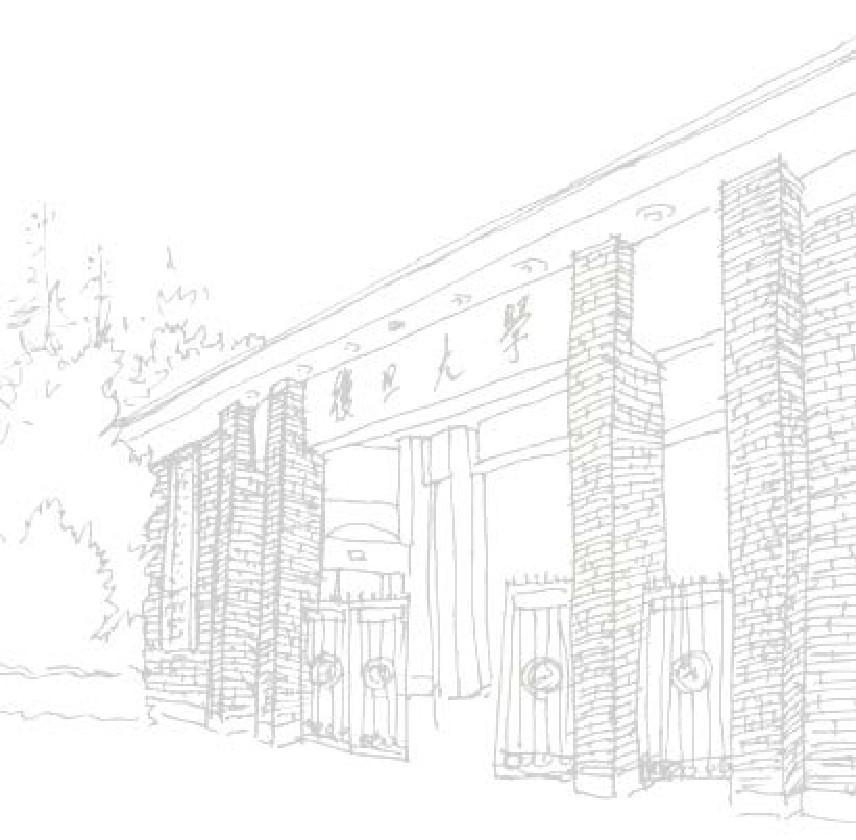
\includegraphics[scale=0.2]{maingate2}}
\begin{document}

\begin{frame}
\titlepage % Print the title page as the first slide
\end{frame}

\begin{frame}
\frametitle{Overview}
\tableofcontents % Throughout your presentation, if you choose to use \section{} and \subsection{} commands, these will automatically be printed on this slide as an overview of your presentation
\end{frame}


%------------------------------------------------
\section{Setting: Two-skill Roy Model} 
%------------------------------------------------

\begin{frame}{Setting: Two-skill Roy Model}
	\begin{itemize}
	\item Income maximizing agents possess two skills $S_1$ and $S_2$ with associated positive skill prices $\pi_1$ and $\pi_2$.
	\pause
	\item Population skill distribution: $F(s_1,s_2)$.
	\pause
	\item Skill $i$ is useful only in sector $i$.
	\pause
	\item An agent chooses sector one if $\pi_1S_1>\pi_2S_2$.
	\pause
	\item Assume that $(S_1,S_2)$ has a well-defined density $f(s_1,s_2)$.
	\pause
	\item The proportion of the population working in sector one is 
	$$P_1=\int^\infty_0\int^{\pi_1S_1/\pi_2}_0f(s_1,s_2)ds_2ds_1.$$
	\end{itemize}
\end{frame}

\begin{frame}{Setting: Two-skill Roy Model}
	\begin{itemize}
	\item The population density of $S_1$ is
	$$f(s_1)=\int^\infty_0f(s_1,s_2)ds_2$$
	\pause
	\item The density  of skill employed in sector one is
	$$g(s_1|\pi_1S_1>\pi_2S_2)=\frac{1}{P_1}\int^{\pi_1S_1/\pi_2}_0f(s_1,s_2)ds_2ds_1$$
	\end{itemize}
\pause
$\Rightarrow$
The distribution of skills observed in sector one differs from the population distribution of skills.
\end{frame}
%我们就是要说明这两个不一样嘛,所以才有自选择的问题。
%------------------------------------------------

\begin{frame}{Setting: Two-skill Roy Model}
	\begin{itemize}
	\item The density of earnings in the economy at large, $g(w)$, is a weighted average of the densities in each sector
	$$g(w)=P_1g_1(w)+P_2g_2(w)$$
	where the weight applied to the sector $i$ density is the proportion of the population in the sector.
	\end{itemize}
\end{frame}


\begin{frame}{Setting: Two-skill Roy Model}
	\begin{itemize}
		\item Define $U_i=lnS_i-\mu_i\quad\Rightarrow\quad lnW_i=ln\pi_i+\mu_i+U_i$

		\item Define
		$$c=ln(\pi_1/\pi_2)+\mu_1-\mu_2,\quad \sigma^2=\sigma_{11}+\sigma_{22}-2\sigma_{12},$$

		$$a_1=\frac{\sigma_{11}-\sigma_{22}}{\sigma^2}, \quad a_2=a_1-1=\frac{-\sigma_{22}+\sigma_{12}}{\sigma^2},$$

		$$D=U_1-U_2, \quad V=a_1U_2-a_2U_1,$$

		$$c_*=c/\sigma,\quad D_*=D/\sigma,$$

		$$\rho=corr[D,U_1]=\frac{\sigma_{11}-\sigma_{12}}{\sigma\sqrt\sigma_{11}}=a_1\sigma/\sqrt\sigma_{11}$$
	\end{itemize}
\end{frame}

\begin{frame}{Setting: Two-skill Roy Model}
Then
	$$U_i=a_iD+V,$$

	$$E[D]=0,\quad E[V]=0,$$

	$$Var[D]=\sigma^2, \quad Var[V]=\frac{\sigma_{11}\sigma_{22}-\sigma_{12}^2}{\sigma^2}=\sigma_{11}(1-\rho^2),$$

	$$Cov[D,V]=0.$$

\end{frame}
%------------------------------------------------
\begin{frame}{Setting: Two-skill Roy Model}
Rewrite the earnings function to be
	\begin{equation}\nonumber
	\begin{aligned}
	lnW_i&=ln\pi_i+\mu_i+a_iD+V \\
	&=ln\pi_i+\mu_i+a_i\sigma D_*+V,
	\end{aligned}
	\end{equation}

\pause
	\begin{equation}\nonumber
		\begin{aligned}
		\Rightarrow lnW_1-lnW_2&=ln\pi_1+\mu_1+a_1D+V-ln\pi_2-\mu_2-a_2D-V \\
		&=c+D=\sigma(c_*+D_*)
		\end{aligned}
	\end{equation}
\end{frame}
%------------------------------------------------
\begin{frame}{Setting: Two-skill Roy Model}
Derive the sectoral moments of log earnings:
	\begin{equation}\nonumber
	\begin{aligned}
	E[lnW_1|lnW_1>lnW_2]&=ln\pi_1+\mu_1+E[U_1|D>-c] \\
	&=ln\pi_1+\mu_1+a_1E[D|D>-c]+E[V|D>-c]
	\end{aligned}
	\end{equation}
and
	\begin{equation}\nonumber
	\begin{aligned}
	Var[lnW_1|lnW_1>lnW_2]=&Var[U_1|D>-c] \\
	=&a^2_1Var[D|D>-c]+Var[V|D>-c] \\
	&+2a_1Cov[D,V|D>-c].
	\end{aligned}
	\end{equation}
\end{frame}
%------------------------------------------------
\begin{frame}{Setting: Two-skill Roy Model}
If $D$ and $V$ are \textit{independent}, then $E[V|D>-c]=0$, $Var[V|D>-c]=Var[V]$ and $Cov[D,V|D>-c]=0$, so

	\begin{equation}\nonumber
	\begin{aligned}
	&E[lnW_1|lnW_1>lnW_2]\\
	&=ln\pi_1+\mu_1+a_1E[D|D>-c] \\
	&=ln\pi_1+\mu_1+a_1\sigma E[D_*|D_*>-c_*],
	\end{aligned}
	\end{equation}
	\begin{equation}\nonumber
	\begin{aligned}
	Var[lnW_1|lnW_1>lnW_2]=&a^2_1Var[D|D>-c]+Var[V] \\
	=&\sigma_{11}(\rho^2Var[D_*|D_*>-c_*]+(1-\rho^2)),
	\end{aligned}
	\end{equation}
and
	\begin{equation}\nonumber
	\begin{aligned}
	&E[(lnW_1-E[lnW_1|lnW_1>lnW_2])^3|lnW_1>lnW_2] \\
	&=a^3_1E[(D-E[D|D>-c])^3|D>-c]+E[V^3] \\
	&=a^3_1\sigma^3E[(D_*-E[D_*|D_*>-c_*])^3|D_*>-c_*]+(1-\rho^2).
	\end{aligned}
	\end{equation}	
\end{frame}
%------------------------------------------------
\begin{frame}{Setting: Two-skill Roy Model}
Likewise, the moments of log skills are:
	\begin{equation}\nonumber
	E[lnS_1|lnW_1>lnW_2]=\mu_1+a_1\sigma E[D_*|D_*>-c_*],
	\end{equation}		
	
	\begin{equation}\nonumber
	Var[lnS_1|lnW_1>lnW_2]=\sigma_{11}(\rho^2Var[D_*|D_*>-c_*]+(1-\rho^2)),
	\end{equation}	
	
	\begin{equation}\nonumber
	\begin{aligned}
	&E[(lnS_1-E[lnS_1|lnW_1>lnW_2])^3|lnW_1>lnW_2] \\
	&=a^3_1\sigma^3E[(D_*-E[D_*|D_*>-c_*])^3|D_*>-c_*]+E[V^3].
	\end{aligned}
	\end{equation}

\end{frame}
%------------------------------------------------
\section{The Roy Model}
%------------------------------------------------
\subsection{Log Concavity and the Roy Model}
\begin{frame}{Log Concavity and the Roy Model}
In this subsection we investigate conditions on $D$ that will allow us to characterize conditional moments. One assumption that will allow us to characterize the truncated distribution of $D$ is that $D$ is \textit{log concave}.
\pause
\bigskip

\textbf{Definition 1:} A \textit{log concave random variable} X is one for which the density $f$ satisties the condition that 

$$f(\lambda x_1+(1-\lambda)x_2)\geq [f(x_1)]^\lambda[f(x_2)]^{1-\lambda},$$

$0\leq\lambda\leq1,$ for $x_1$,$x_2$ in the support of $X$.
\end{frame}
%------------------------------------------------
\begin{frame}{Log Concavity and the Roy Model}
\textbf{Proposition 1:} If $D$ is a \textit{log concave random variable}, then
	
	$$0\leq \frac{\partial E[D|D>d]}{\partial d}\leq 1 $$
	$$0\leq \frac{\partial E[D|D\leq d]}{\partial d}\leq 1 $$
and
	$$\frac{\partial Var[D|D>d]}{\partial d}\leq 0 $$
	$$\frac{\partial Var[D|D\leq d]}{\partial d}\geq 0. $$
\textbf{Corollary 1:} If $D$ is \textit{log concave}, then $Var[D|D\leq d]\leq \sigma^2$.
\end{frame}
%------------------------------------------------
\begin{frame}{Log Concavity and the Roy Model}
The effect of an increase of $\pi_i$ on the mean log skill and earnings in sector one:
\begin{align}\nonumber
	\frac{\partial E[lnW_1|lnW_1>lnW_2]}{\partial ln\pi_i} =\left\{
	\begin{aligned}
		1-a_1\frac{\partial E[D|D>d]}{\partial d}\left|\right._{d=-c} \quad if \quad i=1,\\
		a_1\frac{\partial E[D|D>d]}{\partial d}\left|\right._{d=-c} \quad if \quad i=2,
	\end{aligned}
	\right.
\end{align}
\begin{align}\nonumber
	\frac{\partial E[lnS_1|lnW_1>lnW_2]}{\partial ln\pi_i} =\left\{
	\begin{aligned}
	-a_1\frac{\partial E[D|D>d]}{\partial d}\left|\right._{d=-c} \quad if \quad i=1,\\
	a_1\frac{\partial E[D|D>d]}{\partial d}\left|\right._{d=-c} \quad if \quad i=2.
	\end{aligned}
	\right.
\end{align}

\textbf{Proof:} Recall that
$$c=ln(\pi_1/\pi_2)+\mu_1-\mu_2,$$
$$E[lnW_1|lnW_1>lnW_2]=ln\pi_1+\mu_1+a_1 E[D|D>-c],$$
$$E[lnS_1|lnW_1>lnW_2]=\mu_1+a_1 E[D|D>-c].$$
\hfill $Q.E.D.$
\end{frame}
%------------------------------------------------
\begin{frame}{Log Concavity and the Roy Model}
\textbf{Theorem 1:} If $lnS_1$, $lnS_2$ are joint \textit{log concave} random variables with \textit{log concave} densities, the aggregate log income distribution
	$$ G(lnw)=P_1G_1(lnw)+P_2G_2(lnw) $$
is log concave.

\bigskip
\textbf{Proof:} If $(lnS_1,lnS_2)$ is \textit{log concave} with density $f(lns_1,lns_2)$, then so is $lnW_1,lnW_2$ because translations of \textit{log concave} random variables are \textit{log concave} (Prekopa (1973, Theorem 7)). By the Brascamp-Lieb (1975) theorem, the distribution function $F(lnw_1,lnw_2)$ is \textit{log concave}. The observed wage is $lnW=max(lnW_1,lnW_2)$ with cdf $F(lnw,lnw)$ which is obviously \textit{log concave} if the distribution of $(lnW_1,lnW_2)$ is \textit{log concave}.\hfill $Q.E.D.$
\end{frame}
%------------------------------------------------
\subsection{Consequences of Log Normality}

\begin{frame}{Consequences of Log Normality}
Let $Z$ be a standard \textit{normal} random variable and let $\lambda(d)=E[Z|Z>d]$; then for $d\in (-\infty,\infty)$, we prove the following results:
\begin{itemize}
	\item $\lambda(d)=\frac{\frac{1}{\sqrt {2\pi}} exp\{-d^2/2\}}{\Phi(-d)}>max(0,d)$,
	\item $0<\frac{\partial \lambda(d)}{\partial d}=\lambda'(d)=\lambda(d)(\lambda(d)-d)<1$,
	\item $\frac {\partial^2\lambda(d)}{\partial d^2} > 0$,
	\item $0<Var[Z|Z>d]=1+\lambda(d)d-\lambda^2(d)<1$,
	\item $\frac{\partial Var[Z|Z>d]}{\partial d}<0 $,
	\item $E[(Z-\lambda(d))^3|Z>d]=\lambda(d)(2\lambda^2(d)-3d\lambda(d)+d^2-1)=\frac {\partial^2\lambda(d)}{\partial d^2},$
	\item $E[Z|Z>d]\geq mode[Z|Z>d]$.
\end{itemize}
\end{frame}
%------------------------------------------------
\begin{frame}{Consequences of Log Normality}
Furthermore,
$$lim_{d\to-\infty} \lambda(d)=0, \quad lim_{d\to\infty} \lambda(d)=\infty,$$
$$lim_{d\to-\infty} \frac{\partial\lambda(d)}{\partial d} =0, \quad lim_{d\to\infty} \frac{\partial\lambda(d)}{\partial d} =1,$$
$$lim_{d\to-\infty}Var[Z|Z>d]=1,\quad lim_{d\to\infty}Var[Z|Z>d]=0.$$
\end{frame}

\begin{frame}{Consequences of Log Normality}
	\textbf{Theorem 2:} For a \textit{log normal} Roy economy, any random assignment of persons to sectors with the same proportion of persons in each sector as in the Roy economy has higher variance of log earnings provided the proportions lie strictly in the unit interval. This is true whether or not skill prices in the two economies are the same.
\end{frame}

\begin{frame}
	\textbf{Proof:}
	
	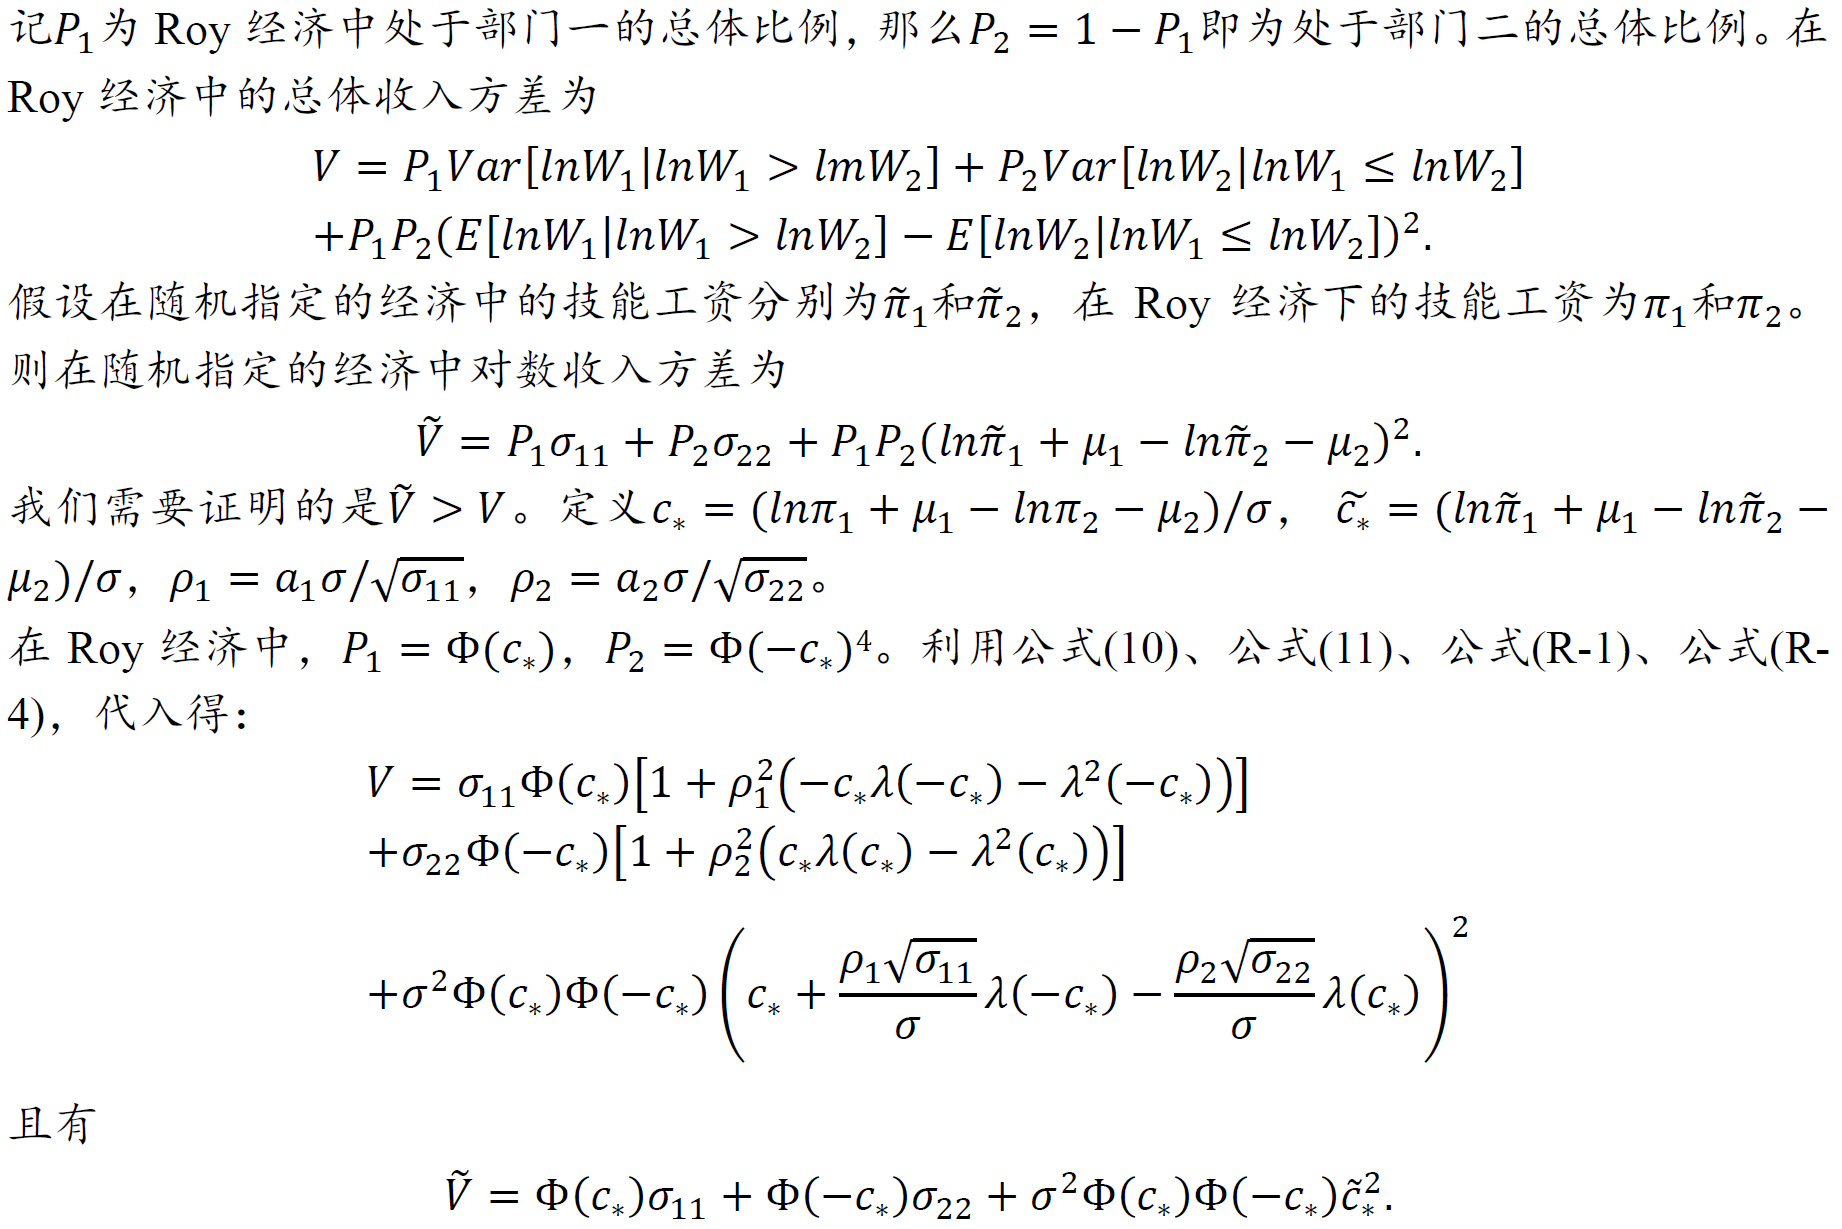
\includegraphics[scale=0.5]{theorem2_1}
	%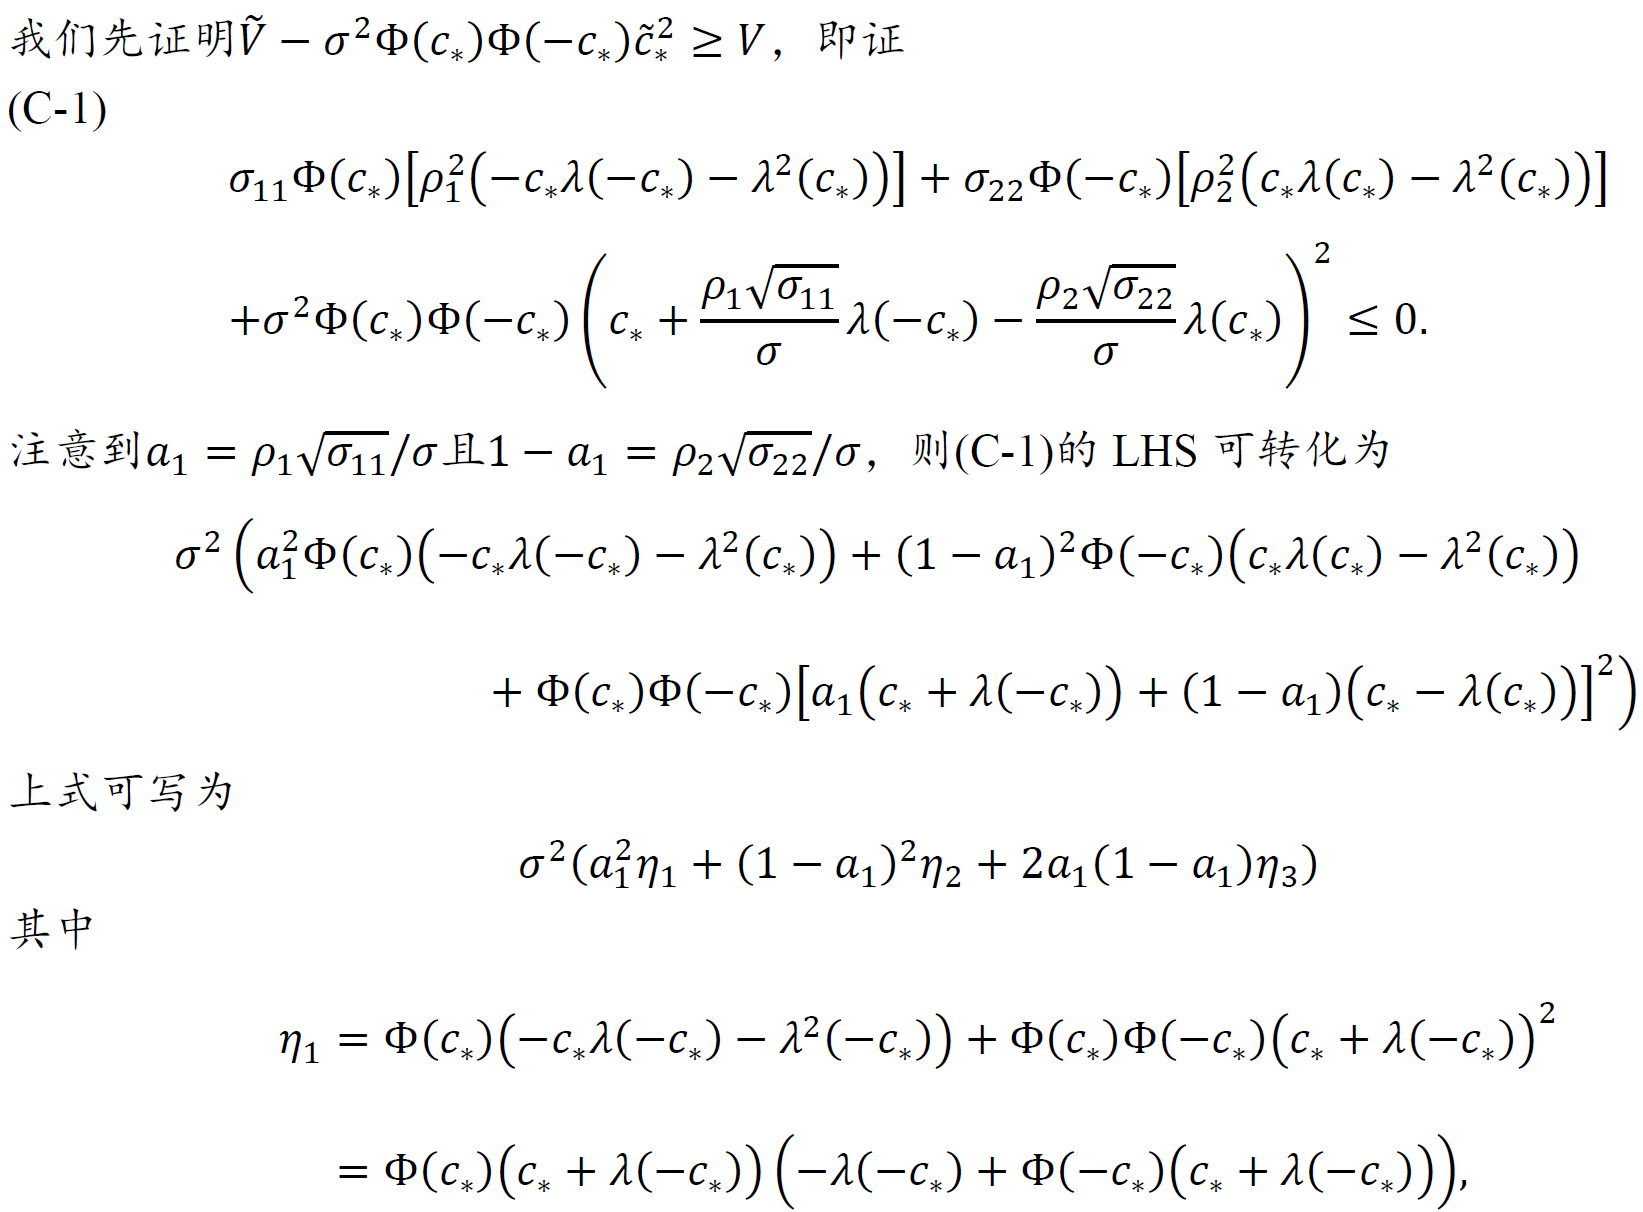
\includegraphics[scale=0.5]{theorem2_2}
\end{frame}
\begin{frame}{Consequences of Log Normality}
	\textbf{Proof:(Cont.)}
	
	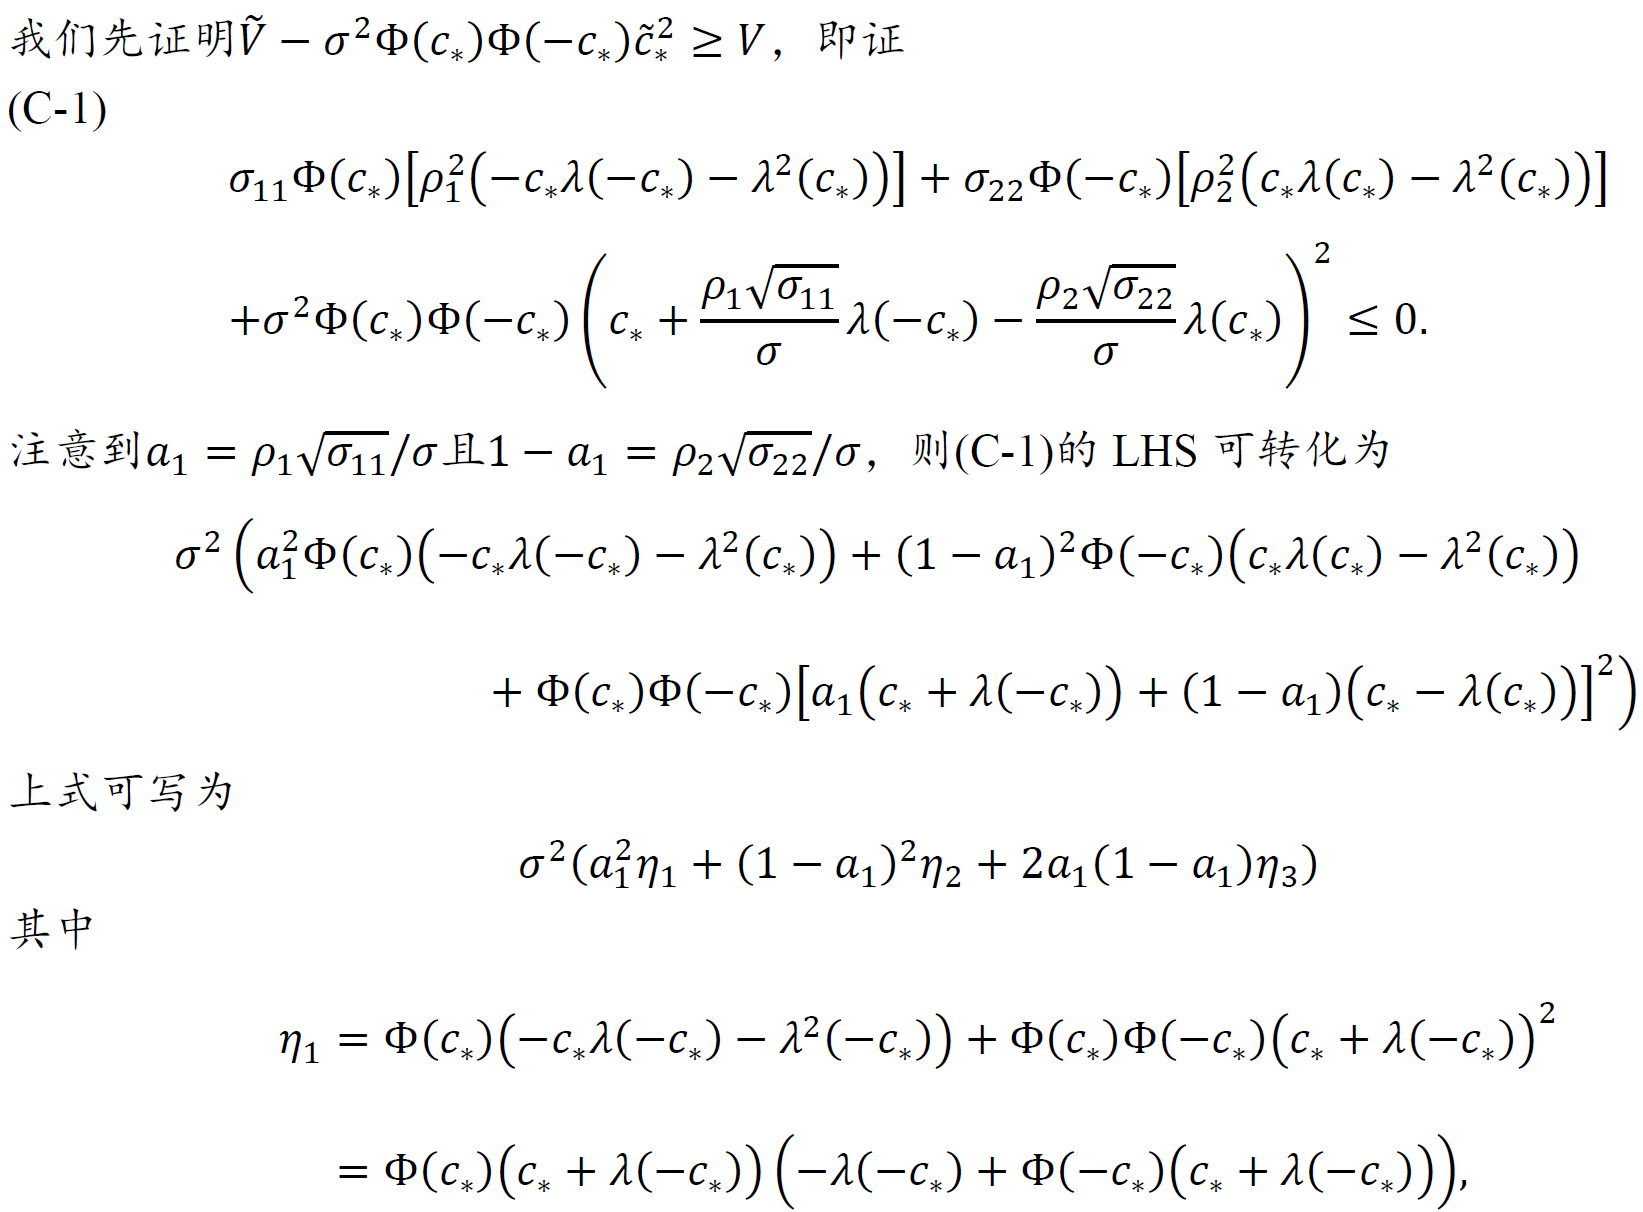
\includegraphics[scale=0.49]{theorem2_2}
\end{frame}
\begin{frame}{Consequences of Log Normality}
	\textbf{Proof:(Cont.)}
	
	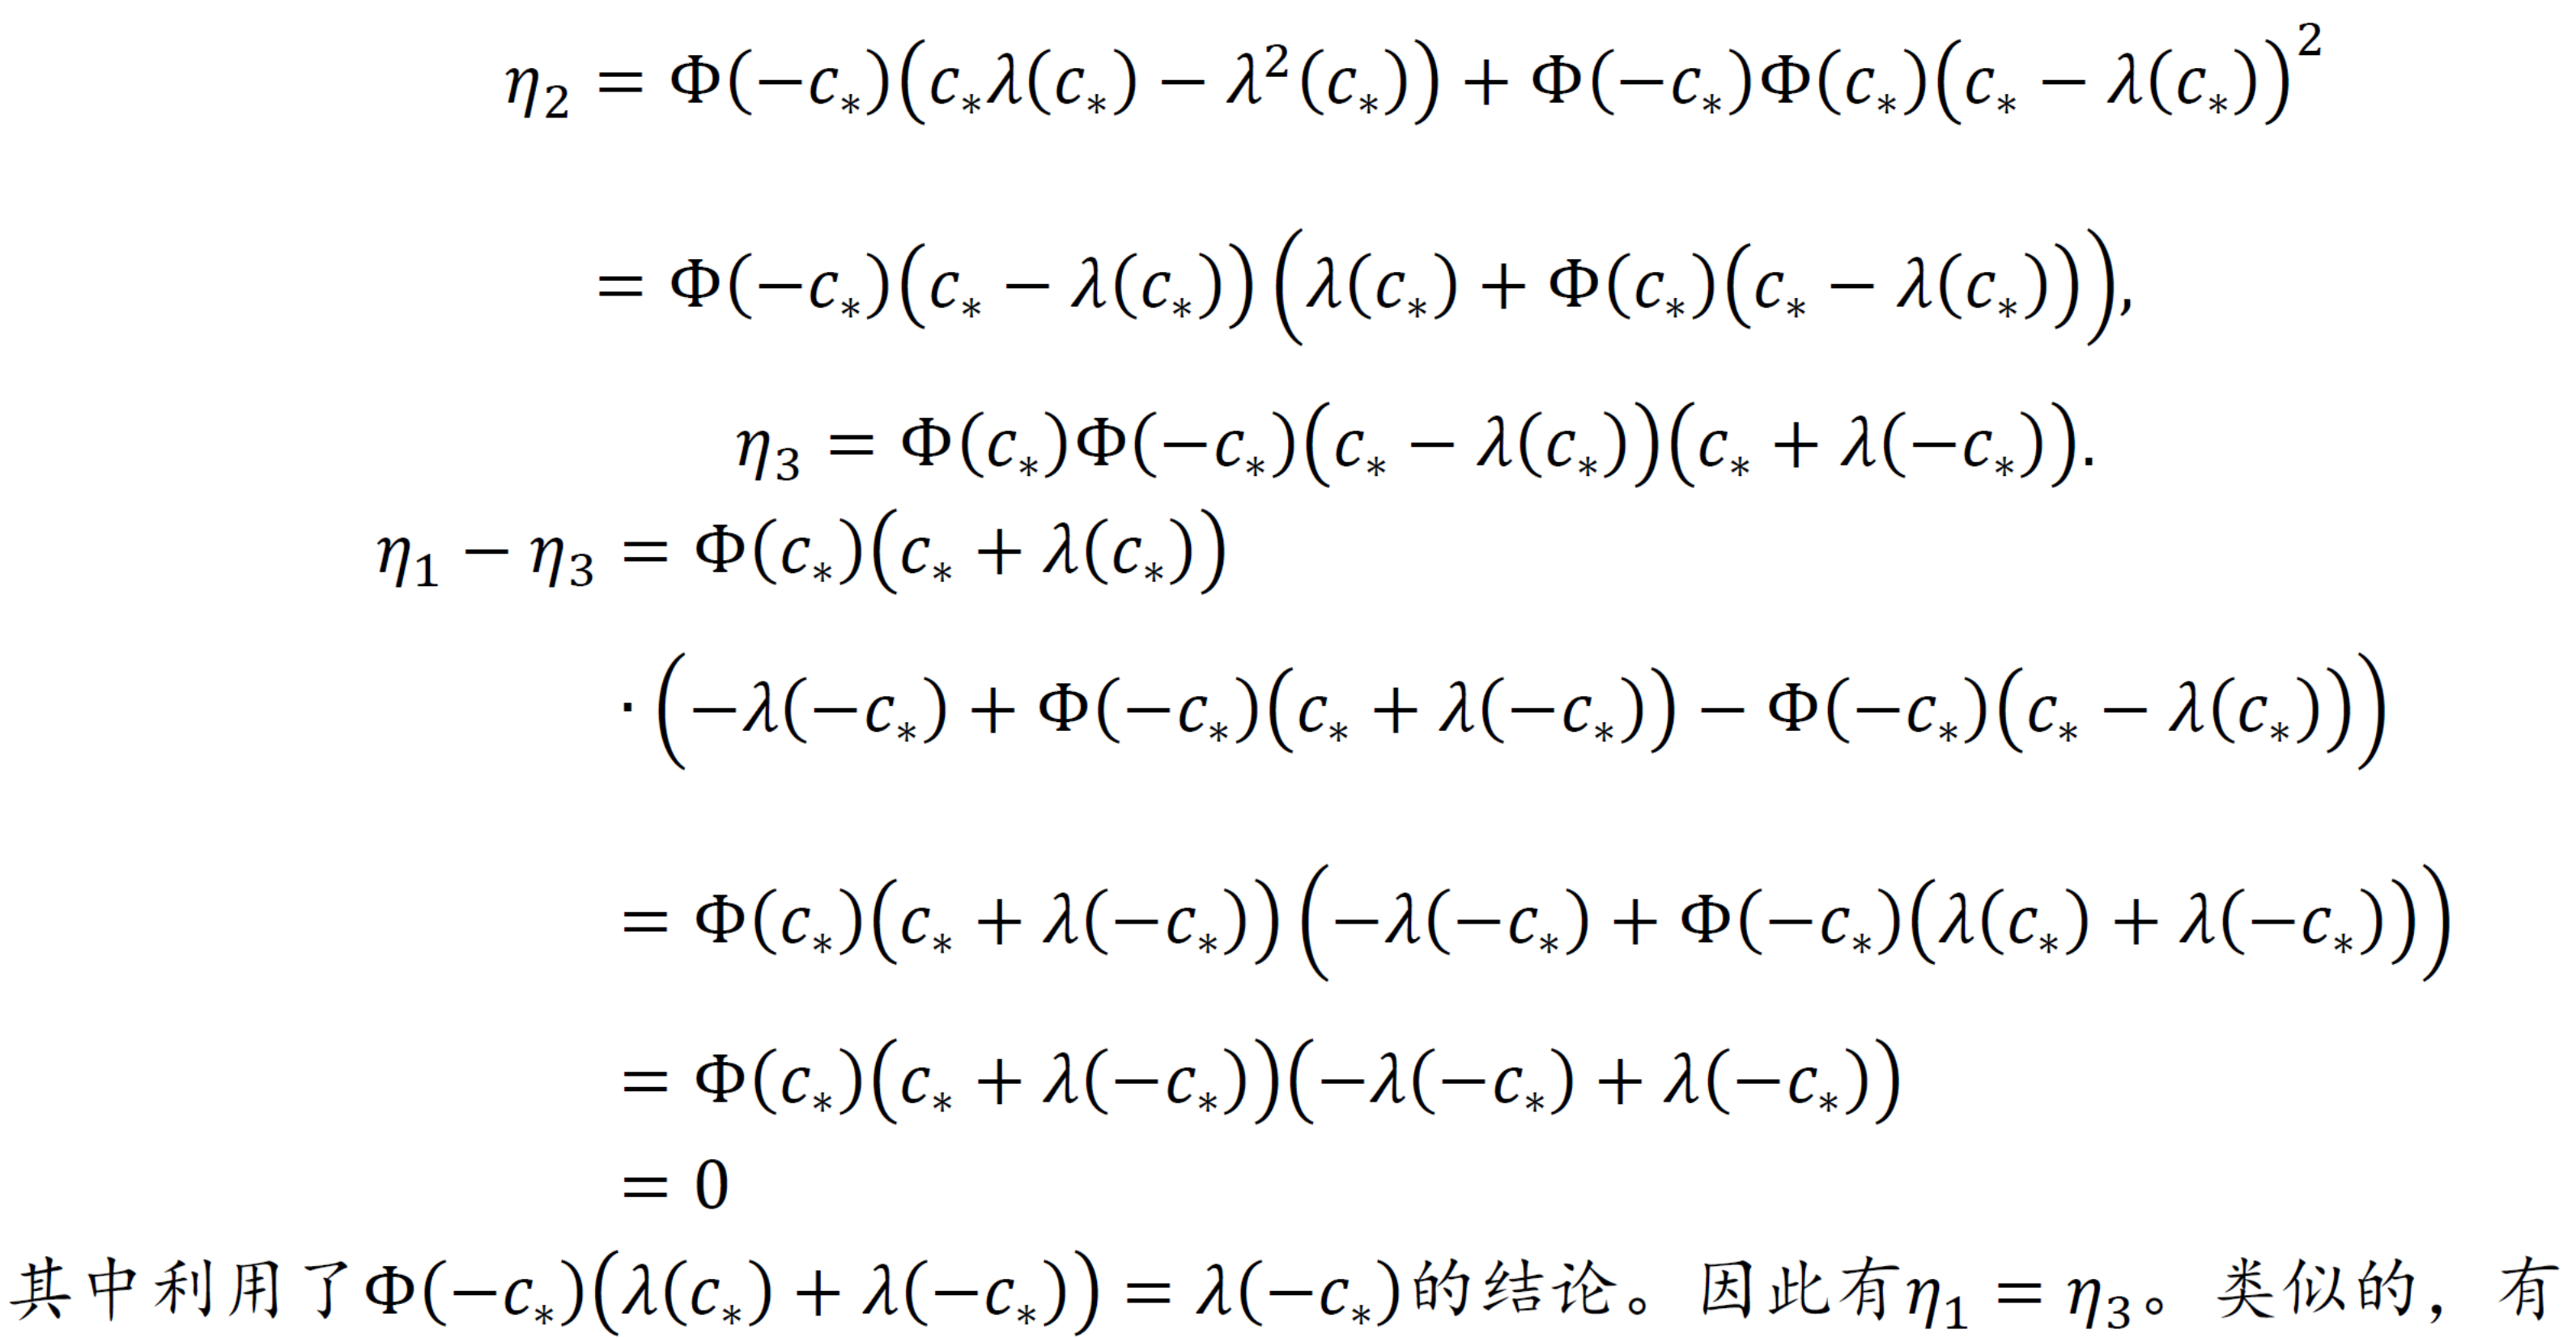
\includegraphics[scale=0.29]{theorem2_3}
\end{frame}
\begin{frame}{Consequences of Log Normality}
	\textbf{Proof:(Cont.)}
	
	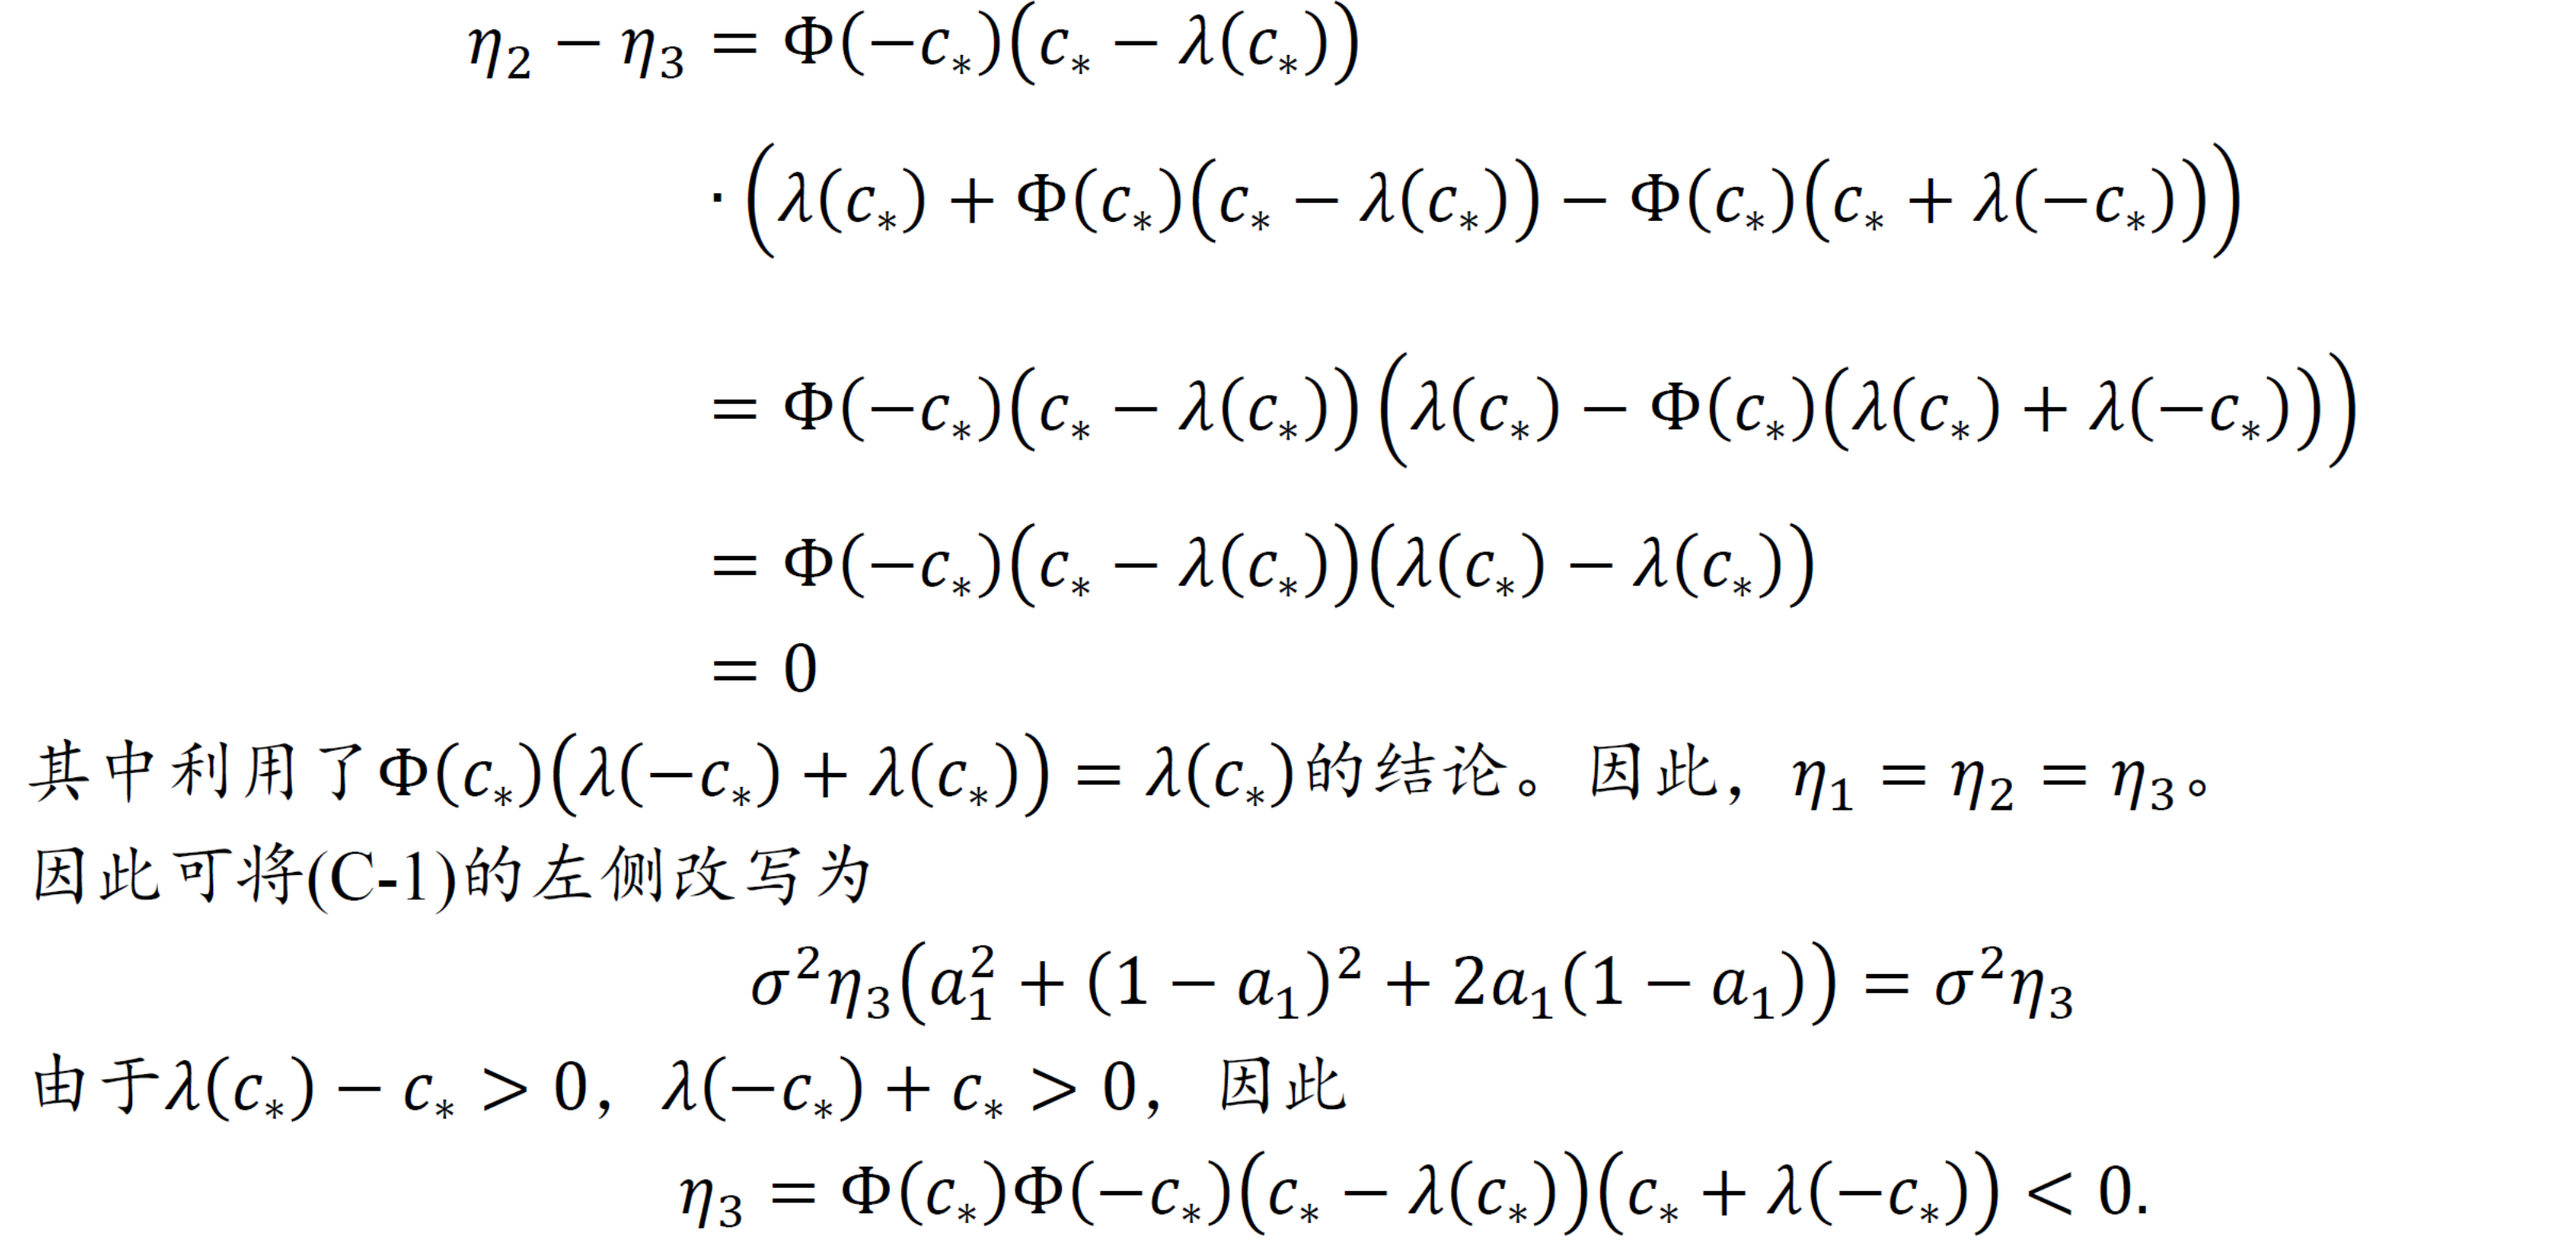
\includegraphics[scale=0.29]{theorem2_4}
\end{frame}
\begin{frame}{Consequences of Log Normality}
	\textbf{Proof:(Cont.)}
	
	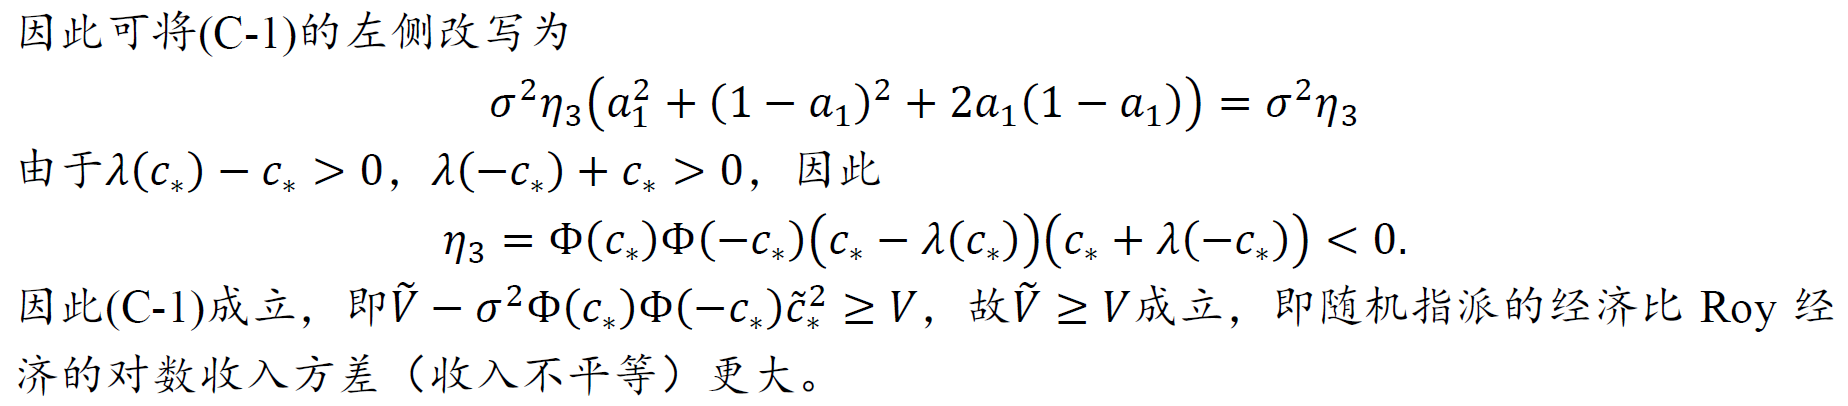
\includegraphics[scale=0.5]{theorem2_5}
	\hfill $Q.E.D$
\end{frame}

\begin{frame}{Consequences of Log Normality}
	\textbf{Theorem 3:} In a \textit{log normal} skill Roy economy, \textcolor{red}{aggregate} log earnings distributions are right skewed as long as some positive fraction of the population works in each sector.

	\bigskip
	Note that
	\begin{itemize}
		\item Sectoral distribution skewness:
	\end{itemize}
	\begin{equation}\nonumber
		\begin{aligned}
		&E[(lnW_1-E[lnW_1|lnW_1>lnW_2])^3|lnW_1>lnW_2] \\
		&=a^3_1E[(D-E[D|D>-c])^3|D>-c]+E[V^3] \\
		&=a^3_1\sigma^3E[(D_*-E[D_*|D_*>-c_*])^3|D_*>-c_*]+(1-\rho^2),
		\end{aligned}
	\end{equation}
	\begin{itemize}
		\item Aggregate distribution skewness:
	\end{itemize}
	$$E[(\max \{lnW_1,lnW_2\}-E[\max \{lnW_1,lnW_2\}])^3].$$

\end{frame}

%------------------------------------------------
\subsection{Nonrobustness of the Roy Model to Non-Log Concavity}
%------------------------------------------------
\begin{frame}{Nonrobustness of the Roy Model to Non-Log Concavity}
It is natural to ask whether the results obtained for \textit{log concave} models can be generalized to all distributions of $(U_1,U_2)$. As might be expected, the answer is "no". For \textit{log convex} random variables, inequalities in Proposition 1 and the Corollary of the Proposition are \textcolor{red}{reversed}.

\bigskip
\pause
\textbf{Definition 2:} A \textit{log convex} random variable is one for which the density of $f$ satisties the condition that 
	$$f(\lambda x_1+(1-\lambda)x_2)\leq [f(x_1)]^\lambda[f(x_2)]^{1-\lambda},$$
	$0\leq\lambda\leq1,$ for $x_1$,$x_2$ in the support of $\mathbf{X}$.
\end{frame}

\begin{frame}{Nonrobustness of the Roy Model to Non-Log Concavity}
	\textbf{Proposition 2:}
	
	If $D$ is a \textit{log convex} random variable and $D\geq 0$, with support in $[0,\infty)$,
	$$\frac{\partial E[D|D>d]}{\partial d}\geq 1$$
	and
	$$\frac{\partial Var[D|D>d]}{\partial d}\geq 0. $$

\bigskip
\pause
\textbf{Corollary 2:}

If $D$ is \textit{log convex} with support in $[0,\infty)$, then $Var[D|D>d]\geq \sigma^2$.
\end{frame}

\begin{frame}{Comparision}
	\begin{columns}
		\column{0.5\textwidth}
		\begin{itemize}
			\item log concave: very good!
		\end{itemize}
		\column{0.5\textwidth}
		\begin{itemize}
			\item log convex: nonrobust :(
		\end{itemize}
	\end{columns}
	\medskip

	\begin{columns}
		\column{0.5\textwidth}
			$$0\leq \frac{\partial E[D|D>d]}{\partial d}\leq 1 $$
			$$0\leq \frac{\partial E[D|D\leq d]}{\partial d}\leq 1 $$
			\medskip
			$$\frac{\partial Var[D|D>d]}{\partial d}\leq 0 $$
			$$\frac{\partial Var[D|D\leq d]}{\partial d}\geq 0, $$
		\column{0.5\textwidth}
			$$\frac{\partial E[D|D>d]}{\partial d}\geq 1$$
			\bigskip
			$$\frac{\partial Var[D|D>d]}{\partial d}\geq 0. $$
	\end{columns}	
\end{frame}


%------------------------------------------------
\section{Identifiability of the Roy Model and Its Normal Extensions} 
%------------------------------------------------
\begin{frame}{Identifiability of the Roy Model and Its Normal Extensions}
Three steps:
	\begin{itemize}
		\item Identification of \textit{log normal Roy model} from \textcolor{red}{cross-section data};
		\item Nonidentifiability of a general \textit{nonnormal Roy model} in a \textcolor{red}{single cross section};
		\item Identification from \textcolor{red}{multi-market data} in a general \textit{nonnormal Roy model}
		\item [-] Pooled cross-section
		\item [-] Panel data
	\end{itemize}
\end{frame}


%------------------------------------------------
\subsection{Identifiability of the Log Normal Roy Model from Cross-Section Data}
\begin{frame}{Identifiability of the Log Normal Roy Model from Cross-Section Data}
We establish that
	\begin{itemize}
		\item {[Theorem 4]} the log normal skills Roy model is identified using \textcolor{red}{a single cross-section} of data on earnings and sectoral choices of agents. Thus it is possible to identify $\mu$ and $\sum$ of Section 1;
		\item {[Theorem 5]} it is possible to identify $\mu$ and $\sum$ except for their subscripts, from the knowledge of \textcolor{red}{aggregate earnings distribution};
		\item {[Theorem 6]} it is possible to recover the distribution of skills \textcolor{red}{when only the proportion working in each sector and the sectoral earnings distribution in one sector} are observed, as occurs in the housewife case where nonmarket output is not observed.
	\end{itemize}
\end{frame}


%------------------------------------------------
\begin{frame}{Identifiability of the Log Normal Roy Model from Cross-Section Data}
	\textbf{Theorem 4:} Under the conditions postulated for the \textit{log normal} Roy model, $\mu$ and $\sum $ can be identified from data on wages paid in each sector and sectoral choices.
\bigskip

\pause
	\textbf{Proof:}
	
	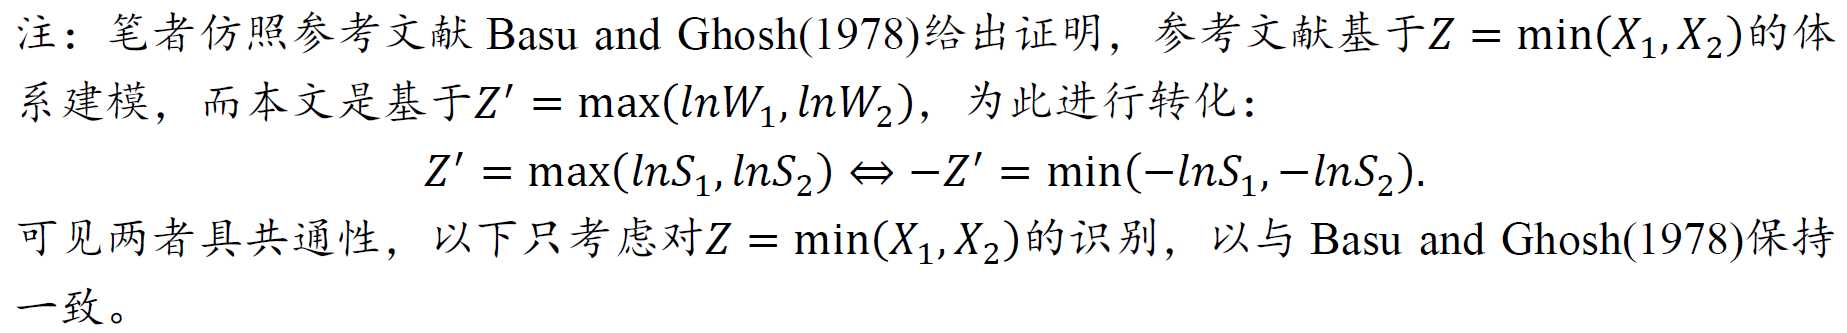
\includegraphics[scale=0.5]{theorem4_0}
\end{frame}
\begin{frame}{Identifiability of the Log Normal Roy Model from Cross-Section Data}
	\textbf{Proof:(Cont.)}
	
	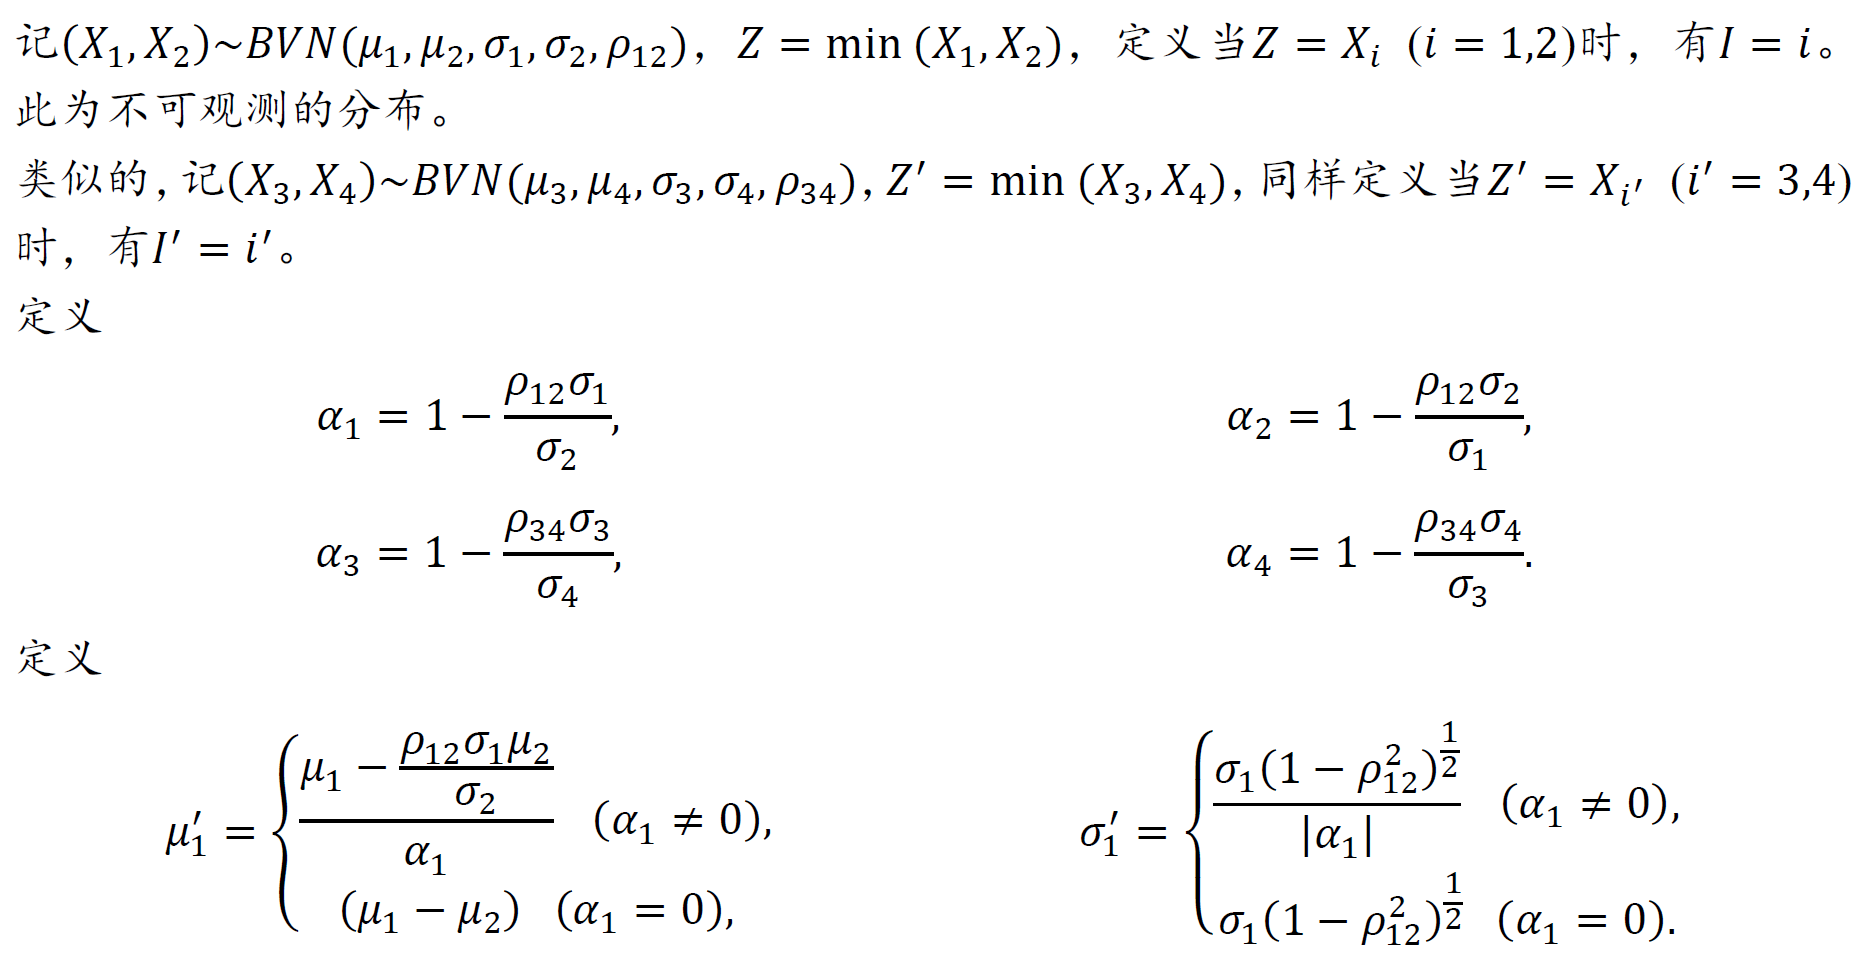
\includegraphics[scale=0.5]{theorem4_1}
\end{frame}
\begin{frame}{Identifiability of the Log Normal Roy Model from Cross-Section Data}
	\textbf{Proof:(Cont.)}
	
	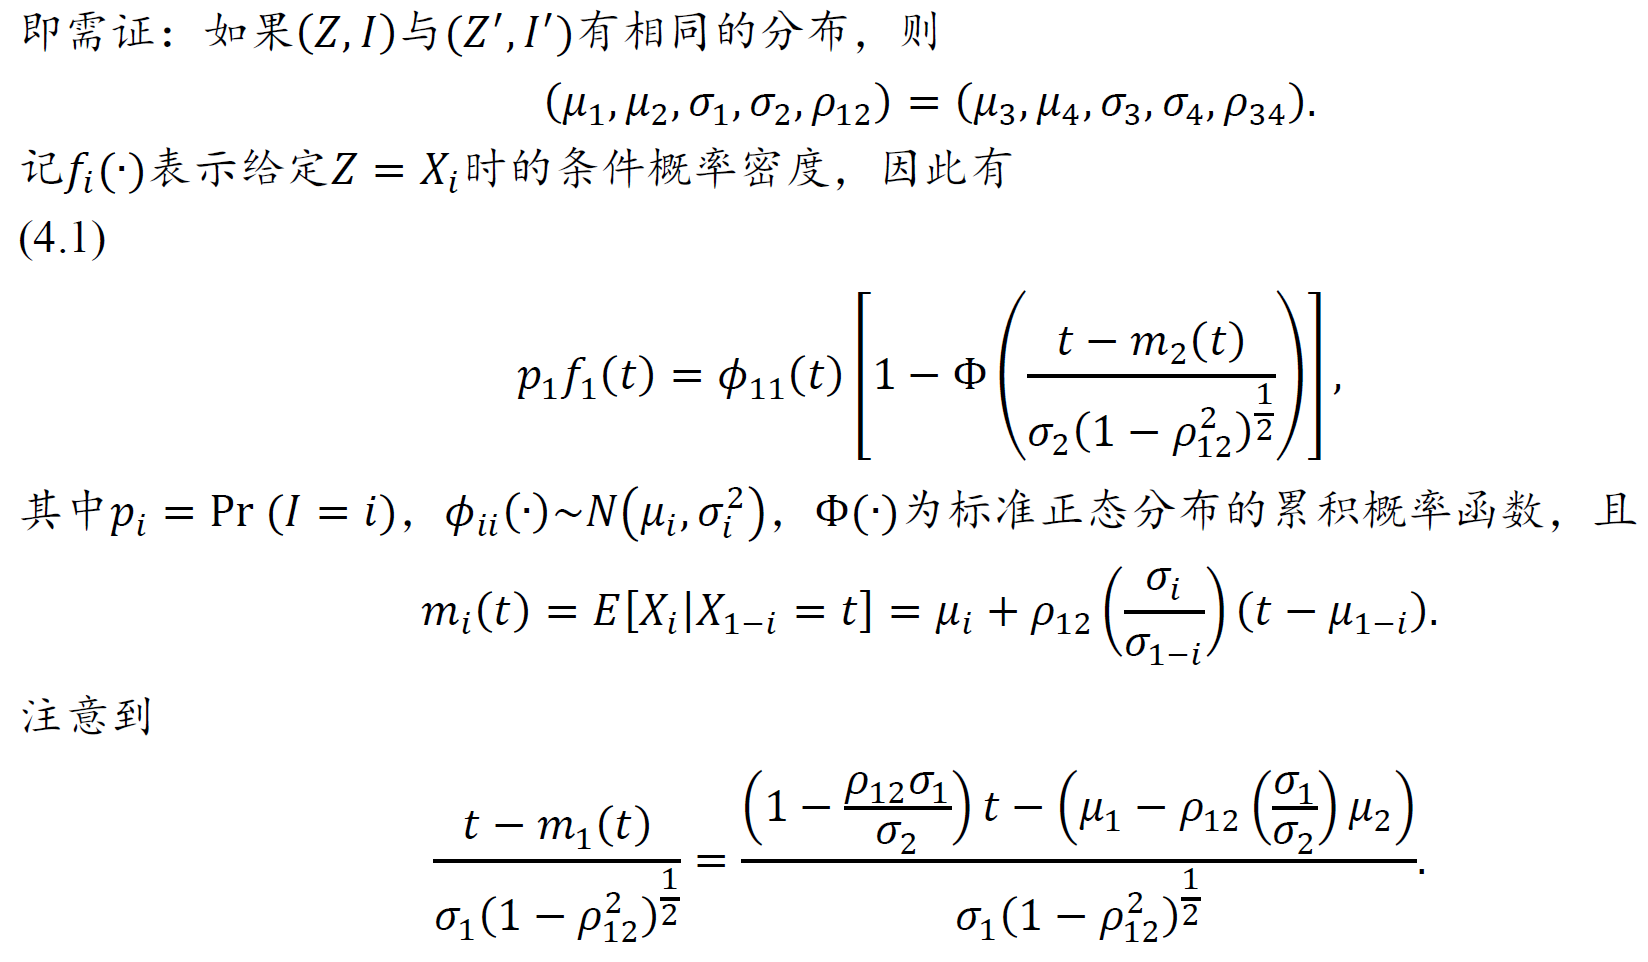
\includegraphics[scale=0.5]{theorem4_2}
\end{frame}
\begin{frame}{Identifiability of the Log Normal Roy Model from Cross-Section Data}
	\textbf{Proof:(Cont.)}
	
	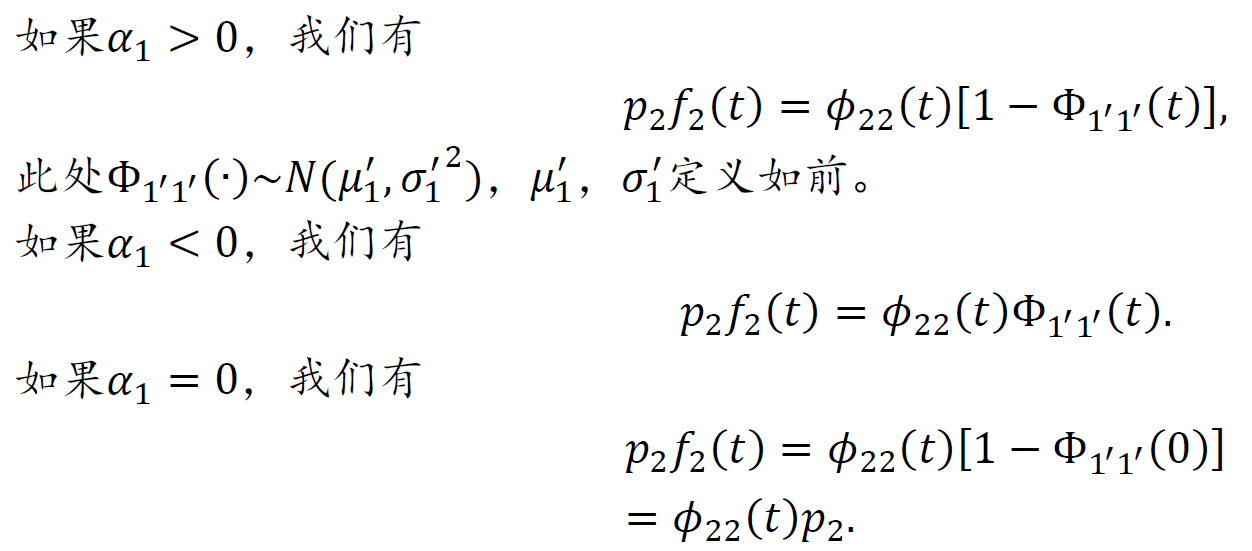
\includegraphics[scale=0.5]{theorem4_3}
\end{frame}
\begin{frame}{Identifiability of the Log Normal Roy Model from Cross-Section Data}
	\textbf{Proof:(Cont.)}
	
	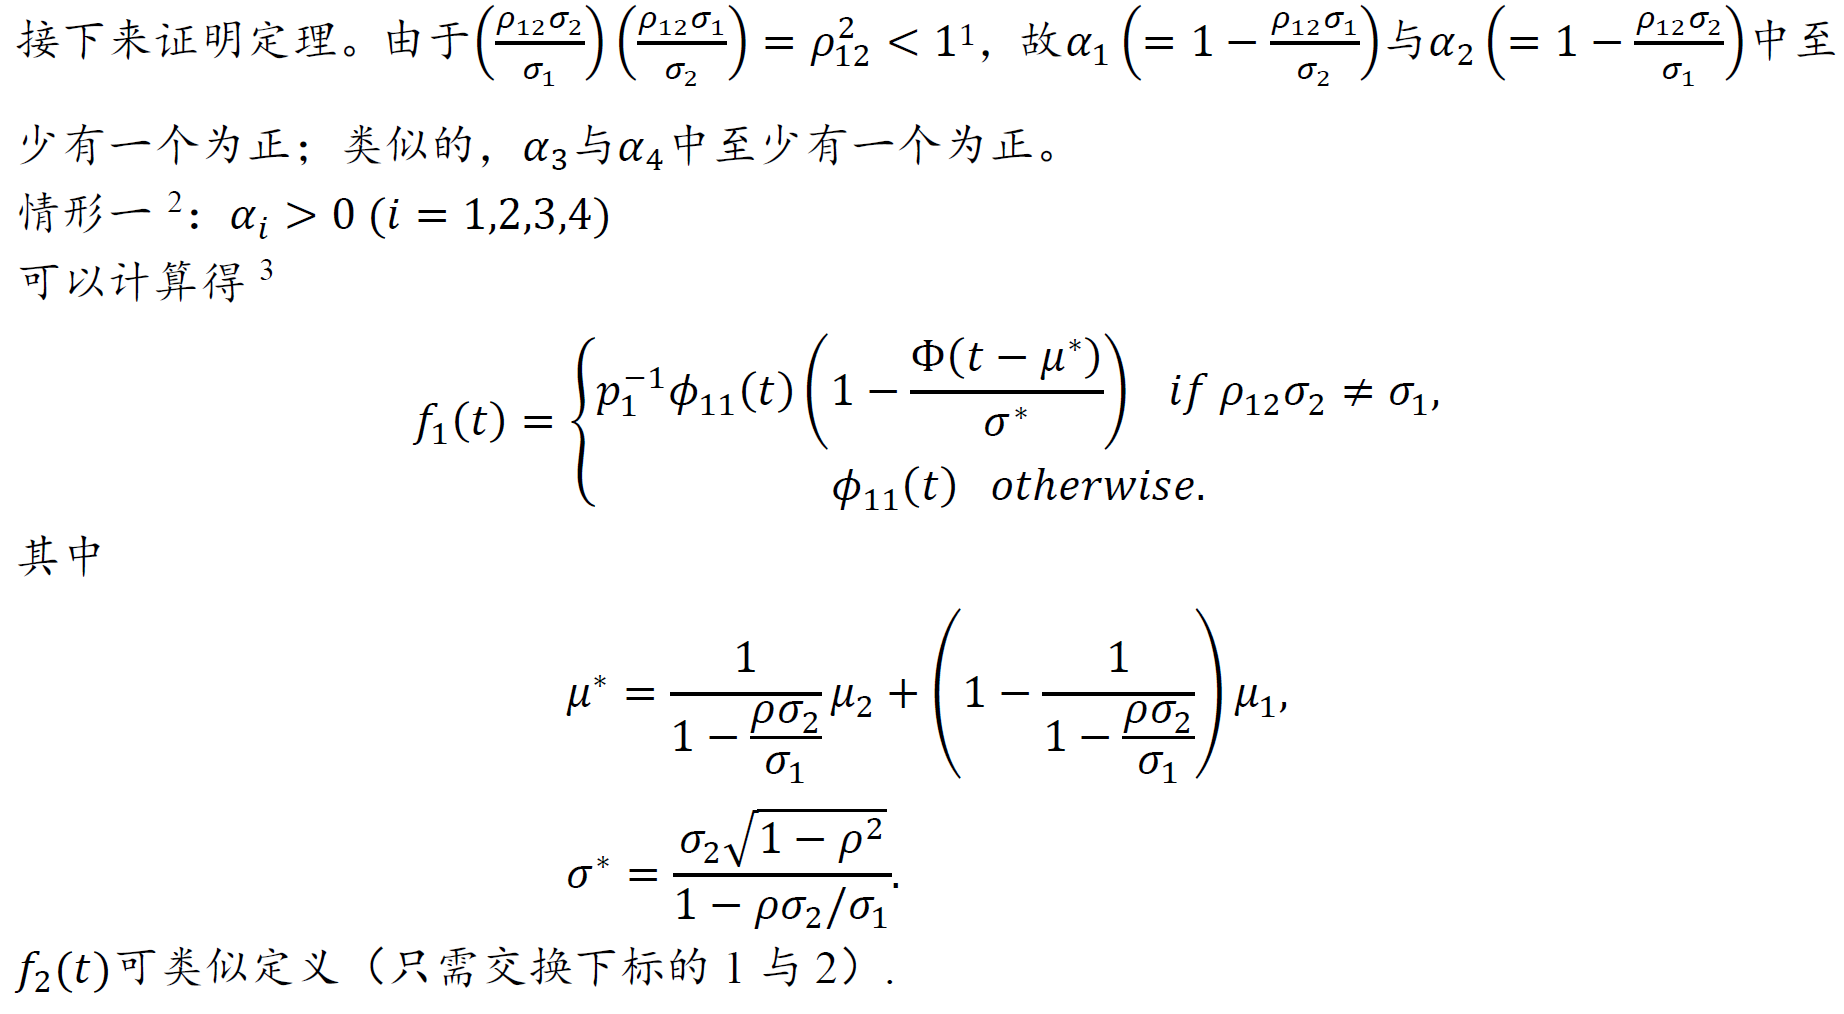
\includegraphics[scale=0.5]{theorem4_4}
\end{frame}
\begin{frame}{Identifiability of the Log Normal Roy Model from Cross-Section Data}
	\textbf{Proof:(Cont.)}
	
	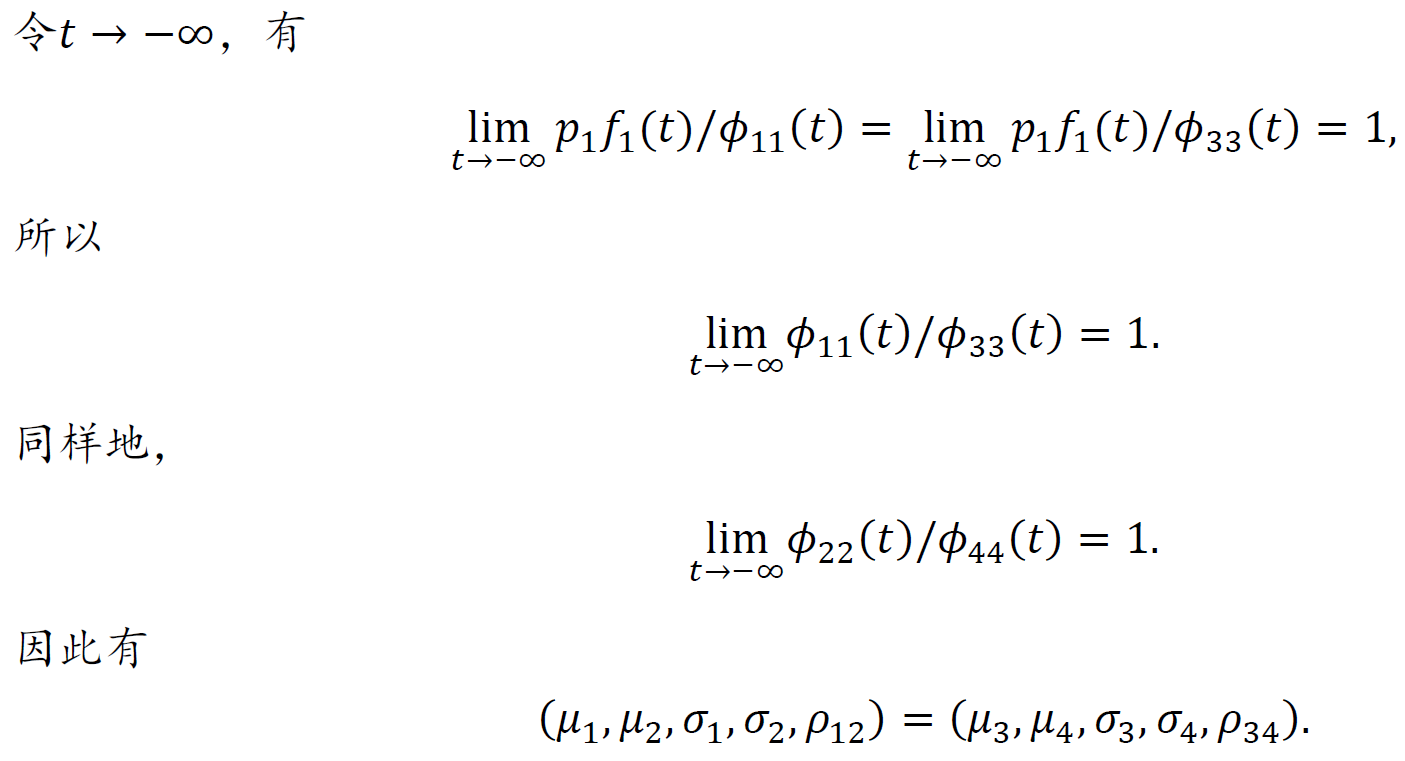
\includegraphics[scale=0.5]{theorem4_5}
\end{frame}
\begin{frame}{Identifiability of the Log Normal Roy Model from Cross-Section Data}
	\textbf{Proof:(Cont.)}
	
	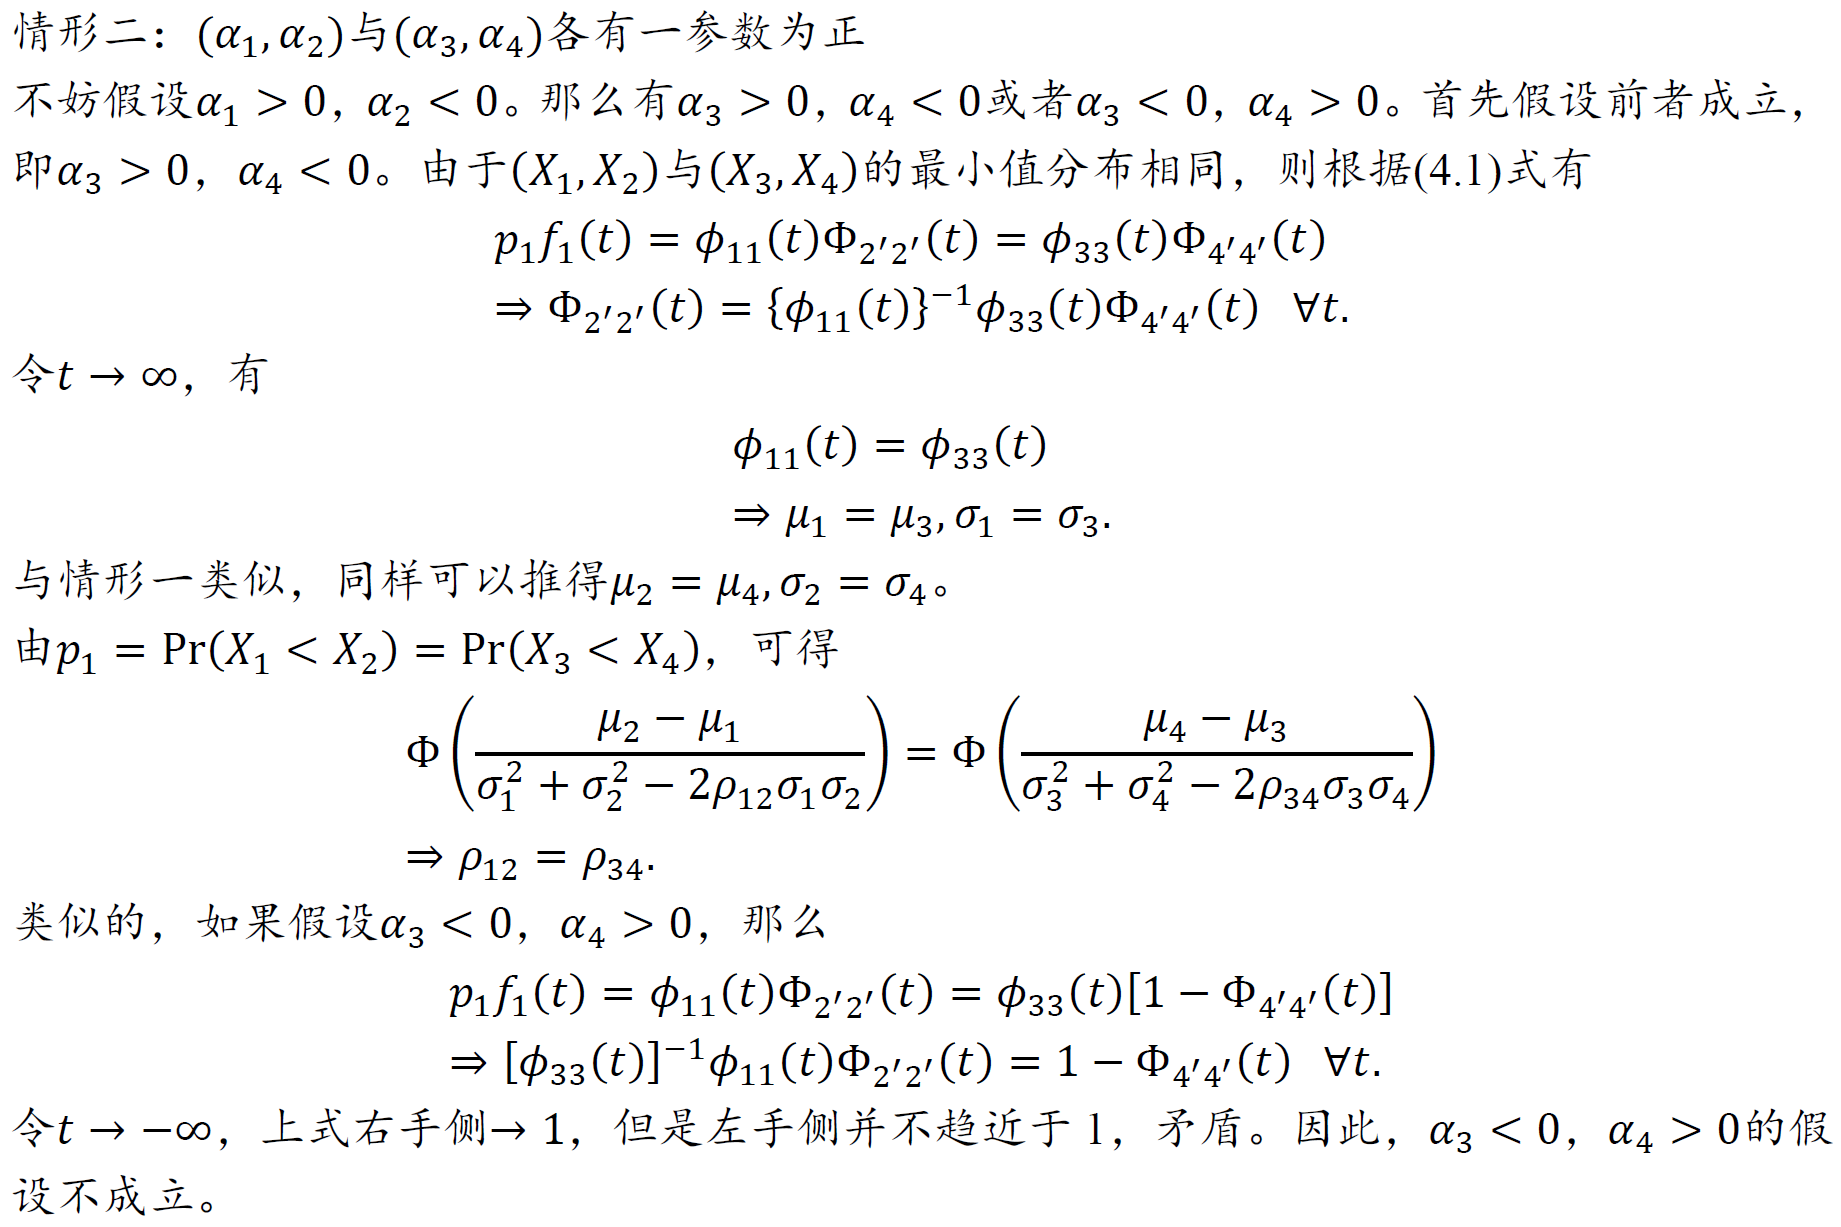
\includegraphics[scale=0.44]{theorem4_6}
\end{frame}
\begin{frame}{Identifiability of the Log Normal Roy Model from Cross-Section Data}
	\textbf{Proof:(Cont.)}
	
	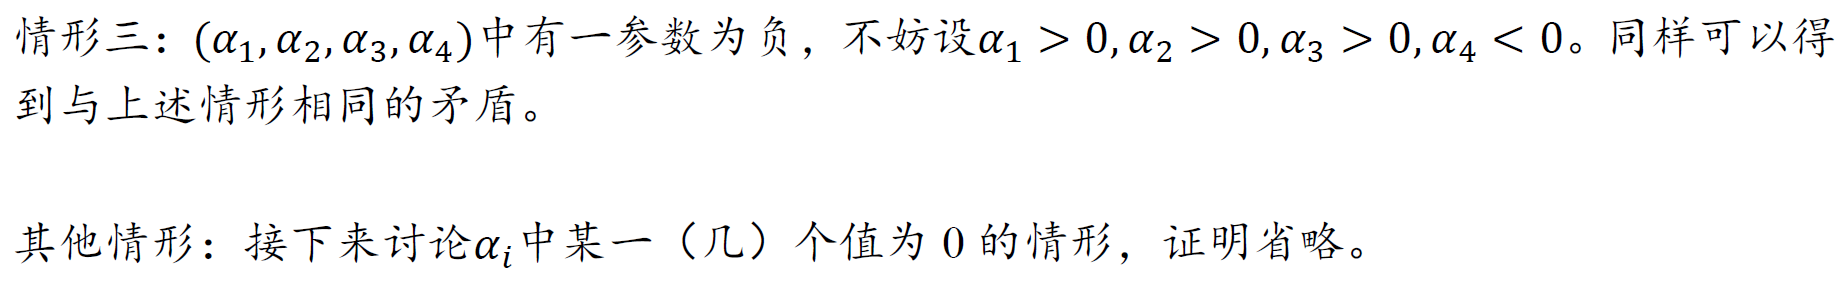
\includegraphics[scale=0.5]{theorem4_7}
	\hfill $Q.E.D.$
\end{frame}

%------------------------------------------------
\begin{frame}{Identifiability of the Log Normal Roy Model from Cross-Section Data}
	\textbf{Theorem 5:} Under the conditions postulated for the \textit{log normal} Roy model, $\mu$ and $\sum $ can be identified, except for their subscripts, from knowledge of the \textcolor{red}{aggregate earnings distribution}.

	\bigskip
	$\Rightarrow$ $\sigma_{12}$ is uniquely identified.
\end{frame}
\begin{frame}{Identifiability of the Log Normal Roy Model from Cross-Section Data}
	\textbf{Proof:}
	
	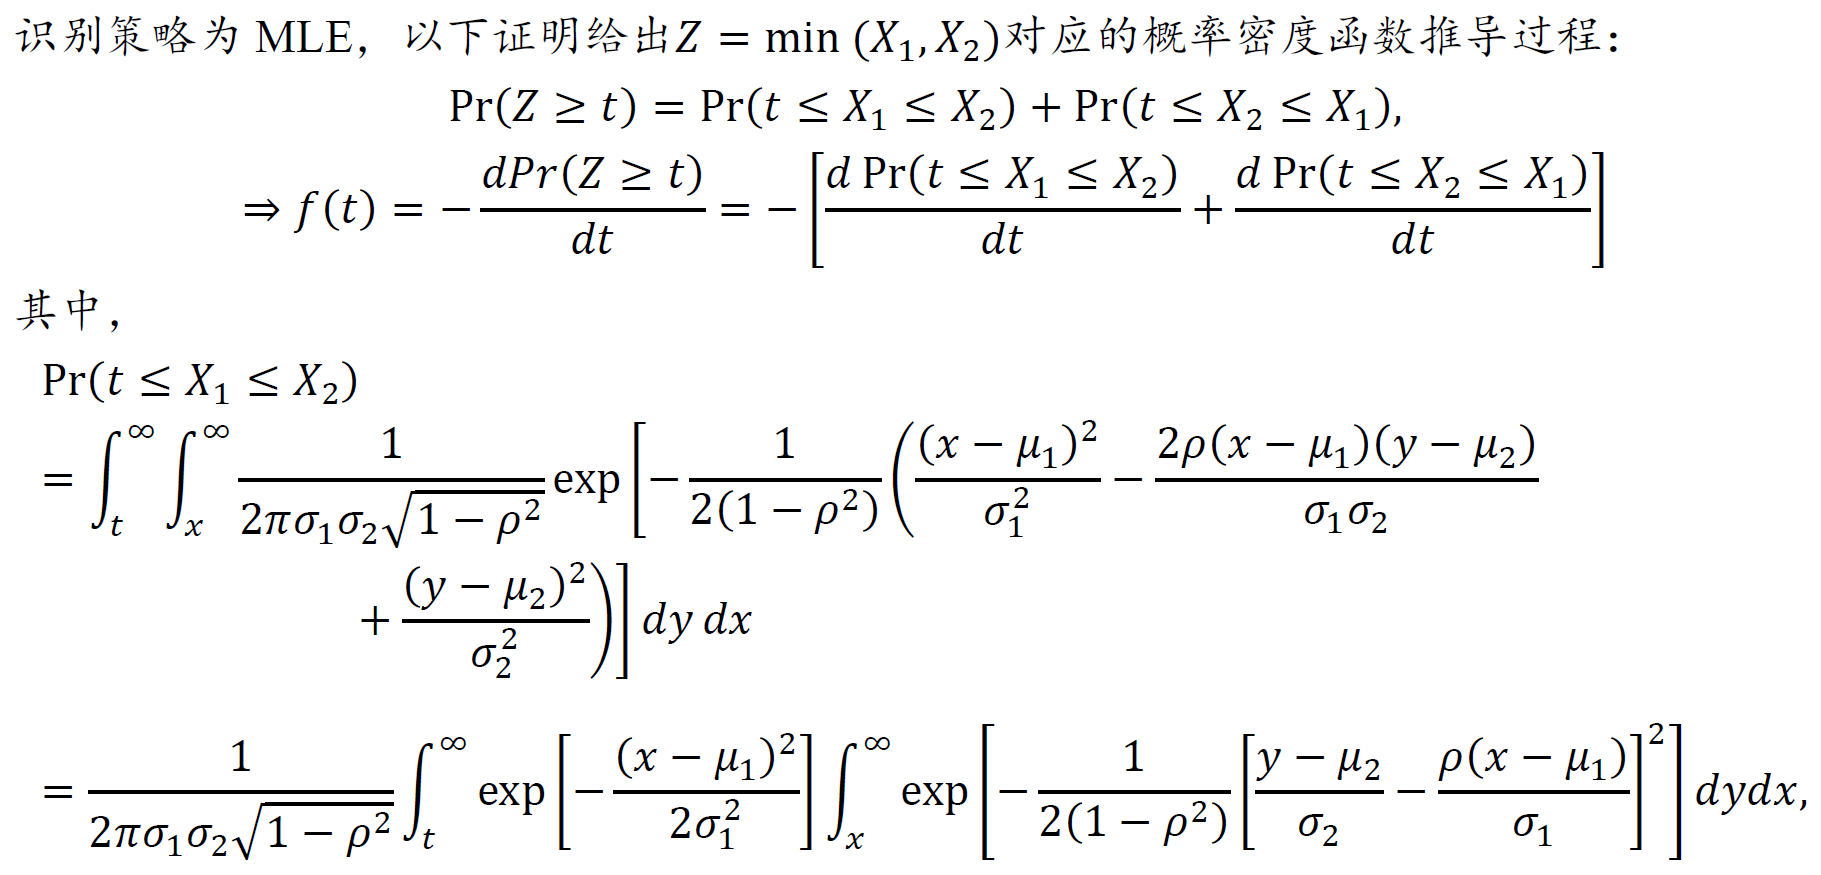
\includegraphics[scale=0.5]{theorem5_1}
\end{frame}
\begin{frame}{Identifiability of the Log Normal Roy Model from Cross-Section Data}
	\textbf{Proof:(Cont.)}
	
	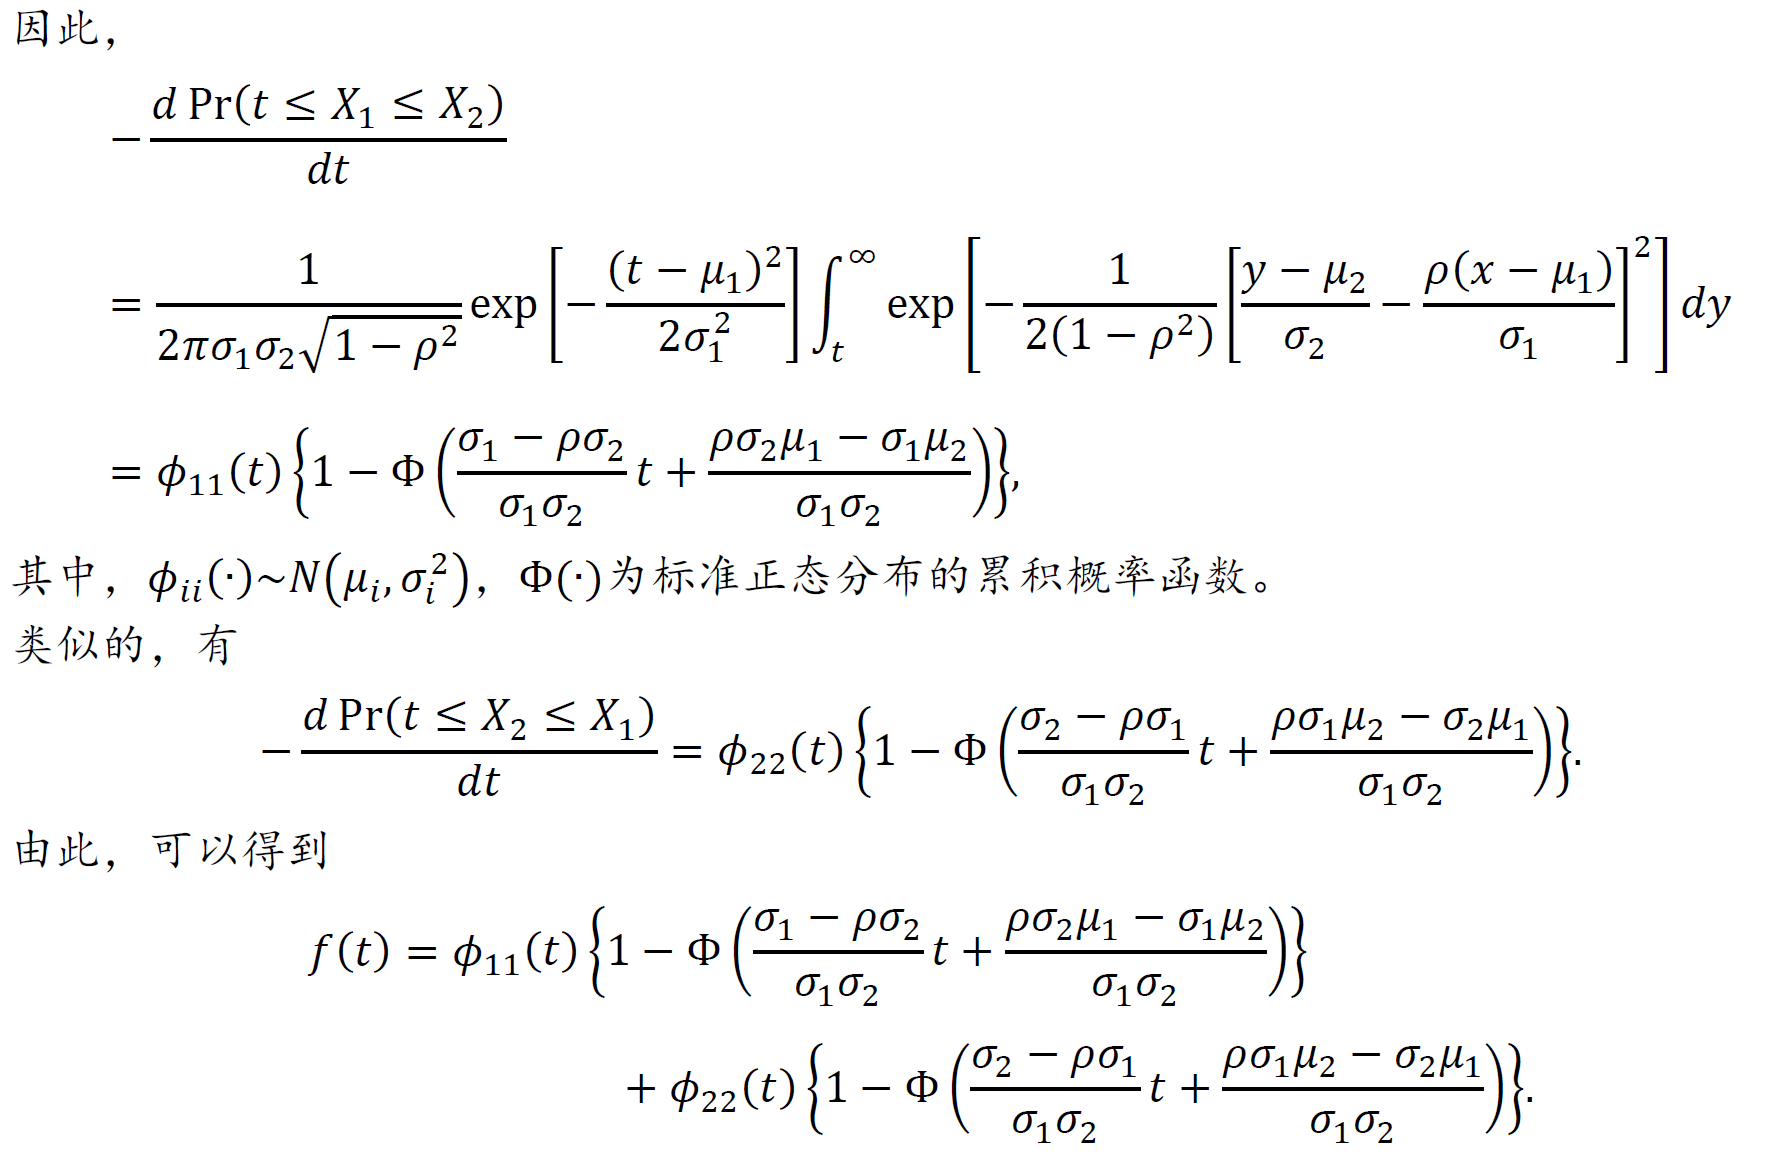
\includegraphics[scale=0.45]{theorem5_2}
\end{frame}
\begin{frame}{Identifiability of the Log Normal Roy Model from Cross-Section Data}
	\textbf{Proof:(Cont.)}
	
	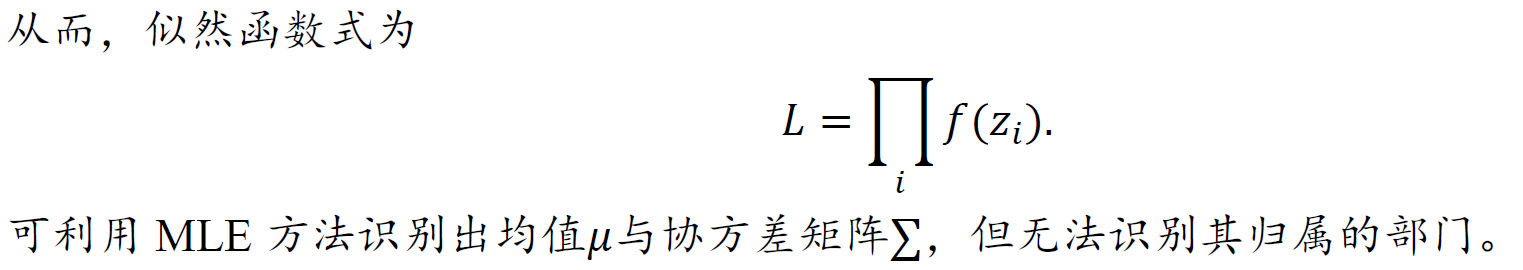
\includegraphics[scale=0.5]{theorem5_3}
\hfill $Q.E.D.$
\end{frame}

\begin{frame}{Identifiability of the Log Normal Roy Model from Cross-Section Data}
	In the analysis of female labor supply, it is often assumed that one of the sectors is home production, where \textcolor{red}{only the proportion working in each sector and the sectoral earnings distribution in one sector} are observed.$\Rightarrow$
	\bigskip

	\textbf{Theorem 6:}	If only the earnings density in sector one, $f(lnw_1 |lnW_1>lnW_2)$ and $Pr(lnW_1>lnW_2)$ are known in the \textit{log normal} Roy model, it is possible to identify $\mu_1$ and $\sigma_{11}$. It is also possible to identify $(\mu_1-\mu_2)/\sigma$ and $\rho$, where $\sigma$ and $\rho$ are as defined in Section 1. Without further restrictions it is not possible to identify $\mu_2$ or $\sigma$.
\end{frame}
\begin{frame}{Identifiability of the Log Normal Roy Model from Cross-Section Data}
	\textbf{Proof:}
	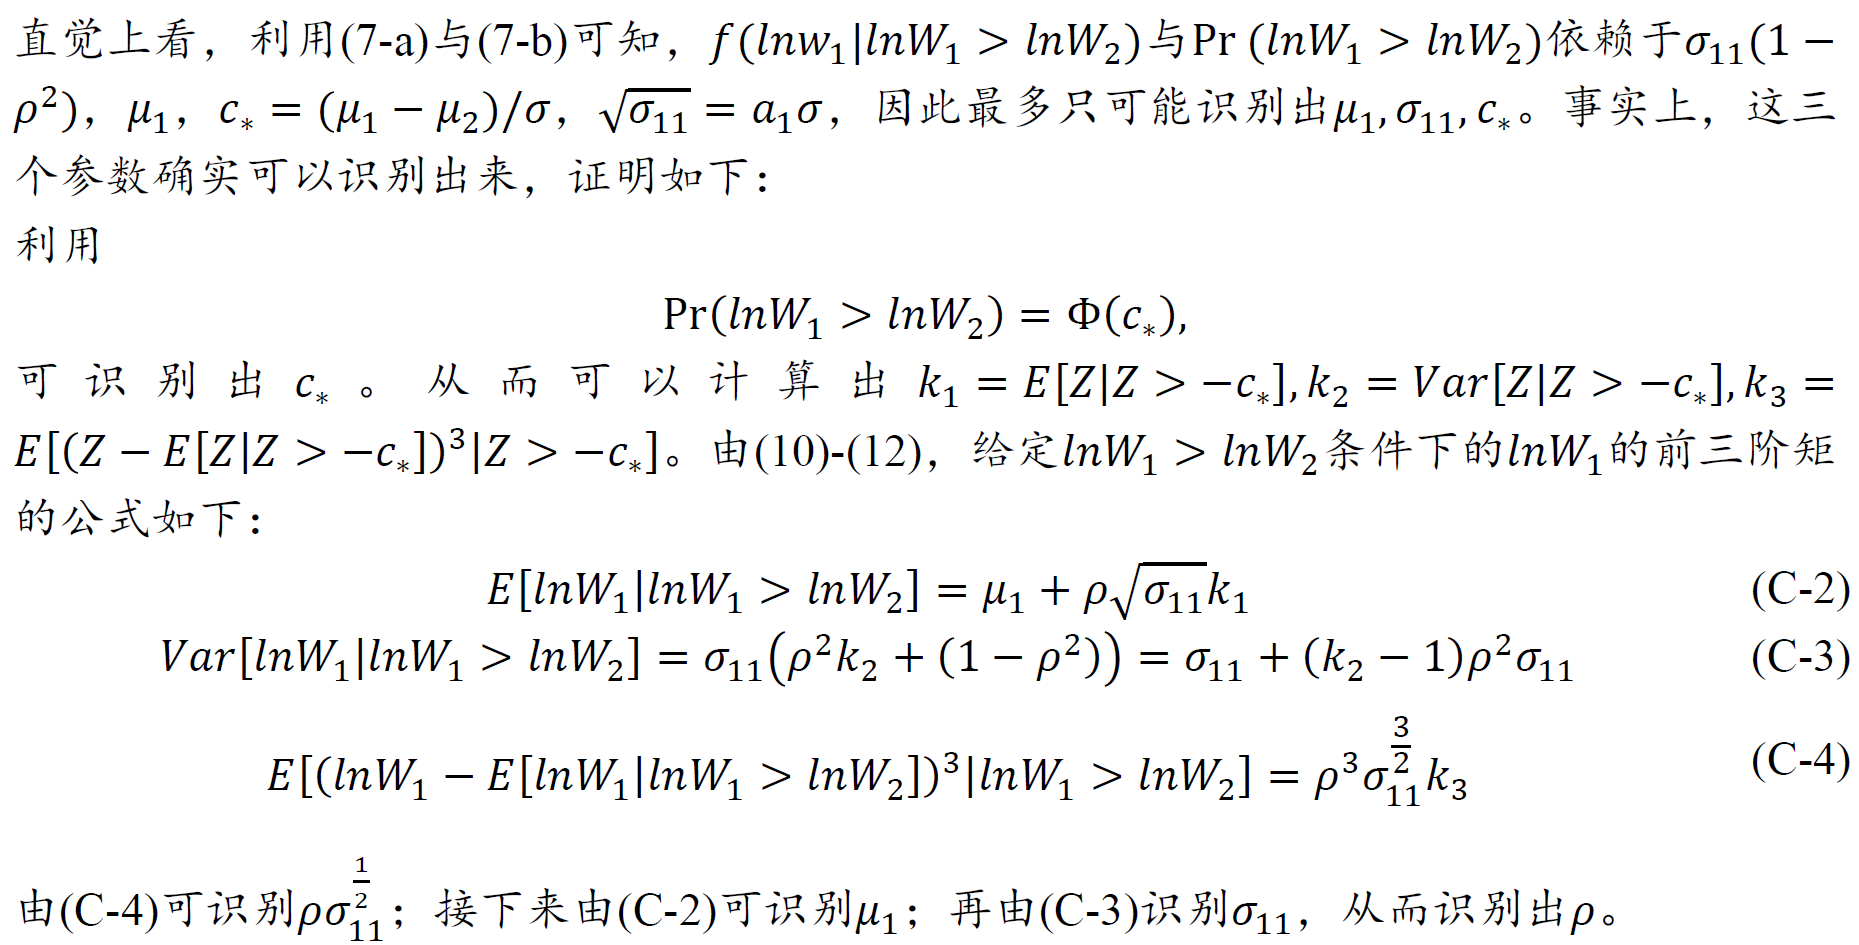
\includegraphics[scale=0.5]{theorem6}
\hfill $Q.E.D.$
\end{frame}

%------------------------------------------------
\subsection{Nonidentifiability of a General Nonnormal Roy Model in a Single Cross Section}
\begin{frame}{The Nonidentifiability of a General Nonnormal Roy Model in a Single Cross Section}
	The results above are not robust when examined in the context of a general \textit{nonnormal} model of skill distribution.
	\medskip
	\pause
	\begin{itemize}
		\item Any cross-section wage distribution can be rationalized by a model with \textcolor{red}{two independent skills} ([Theorem 7]) or \textcolor{red}{two highly correlated skills} ([Theorem 8]). 
	\end{itemize}
\end{frame}


\begin{frame}{Nonidentifiability of a General Nonnormal Roy Model in a Single Cross Section}
	\textbf{Theorem 7:} It is possible to rationalize sectoral wage data in a single cross-section by a \textcolor{red}{two-skill model with independence}. More precisely, it is possible to rationalize data on $f(s_1|S_1>S_2)$, $f(s_2 |S_2>S_1)$, and $P(S_1>S_2)$ by an \textcolor{red}{independent} skill model $f(s_1,s_2 )=f_1 (s_1) f_2 (s_2)$.
\end{frame}
\begin{frame}{Nonidentifiability of a General Nonnormal Roy Model in a Single Cross Section}
\textbf{Proof:}

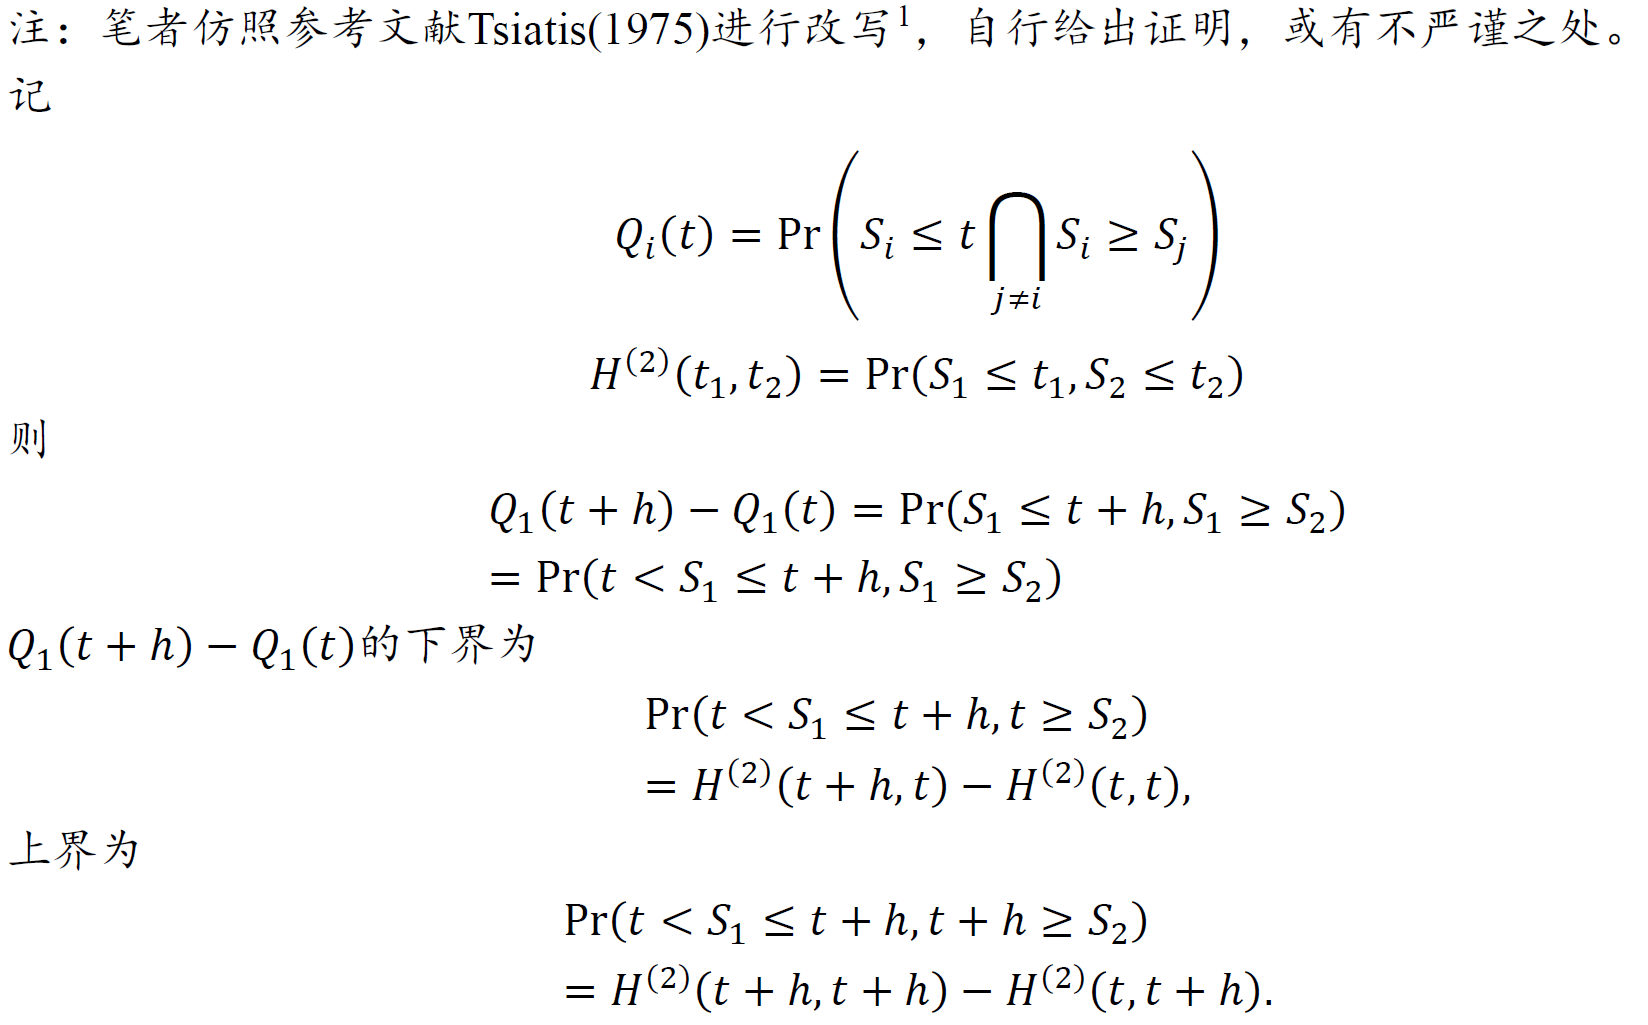
\includegraphics[scale=0.5]{theorem7_1}
\end{frame}
\begin{frame}{Nonidentifiability of a General Nonnormal Roy Model in a Single Cross Section}
	\textbf{Proof:(Cont.)}
	
	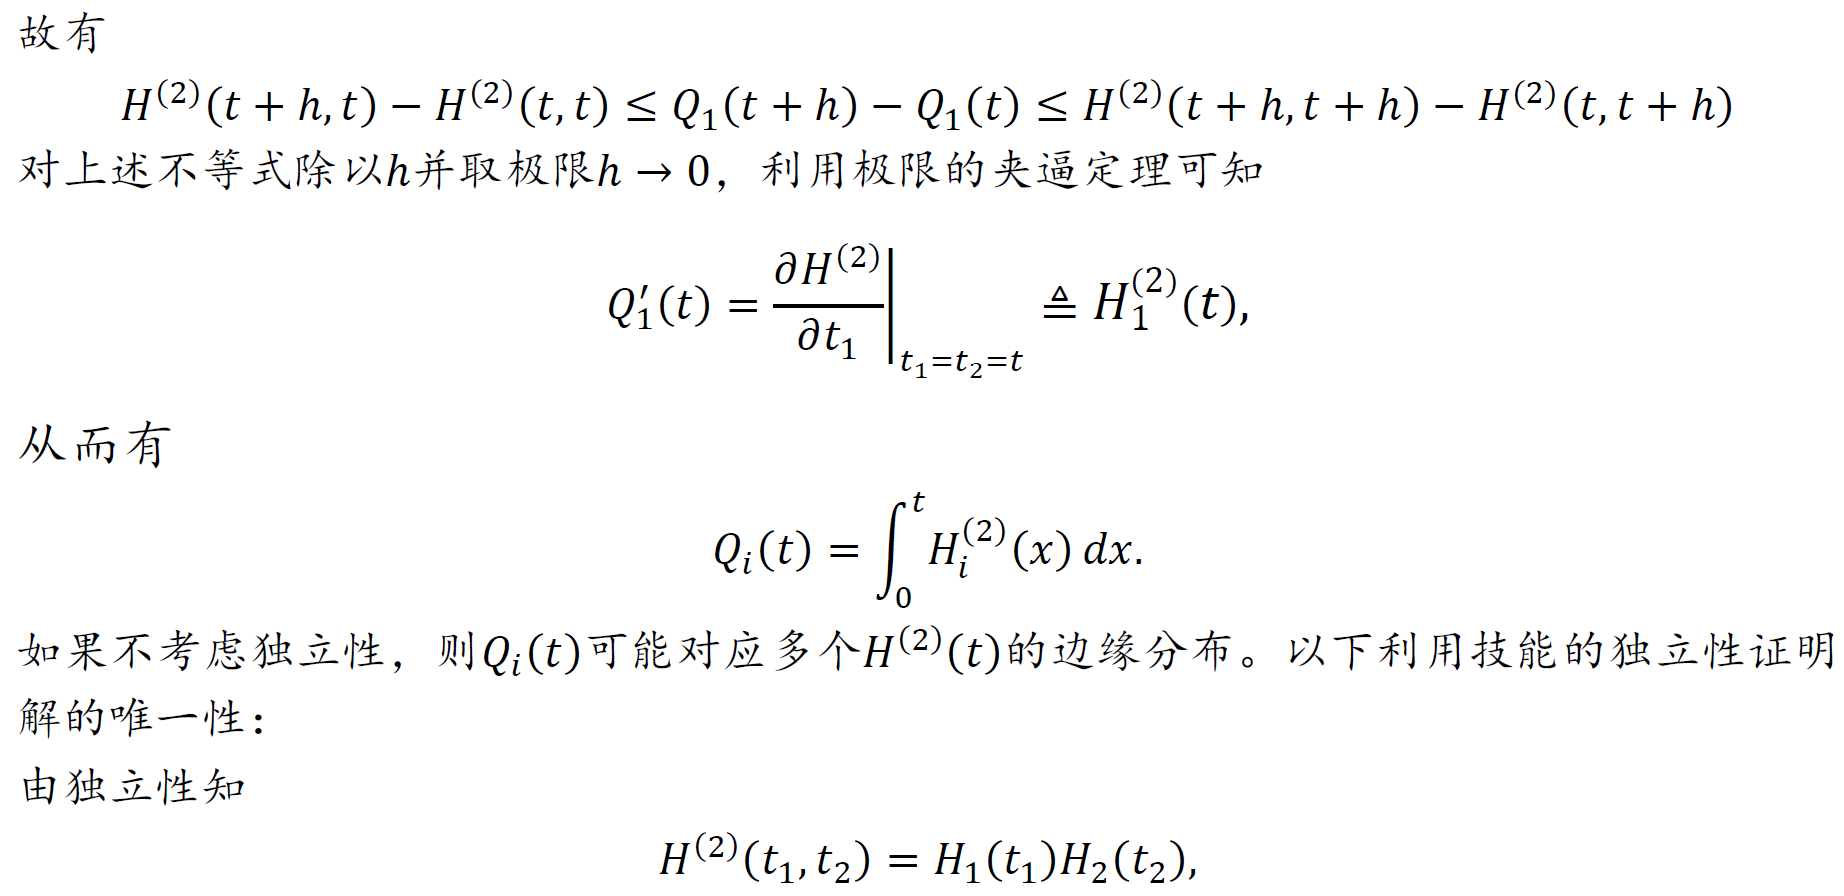
\includegraphics[scale=0.5]{theorem7_2}
\end{frame}
\begin{frame}{Nonidentifiability of a General Nonnormal Roy Model in a Single Cross Section}
	\textbf{Proof:(Cont.)}
	
	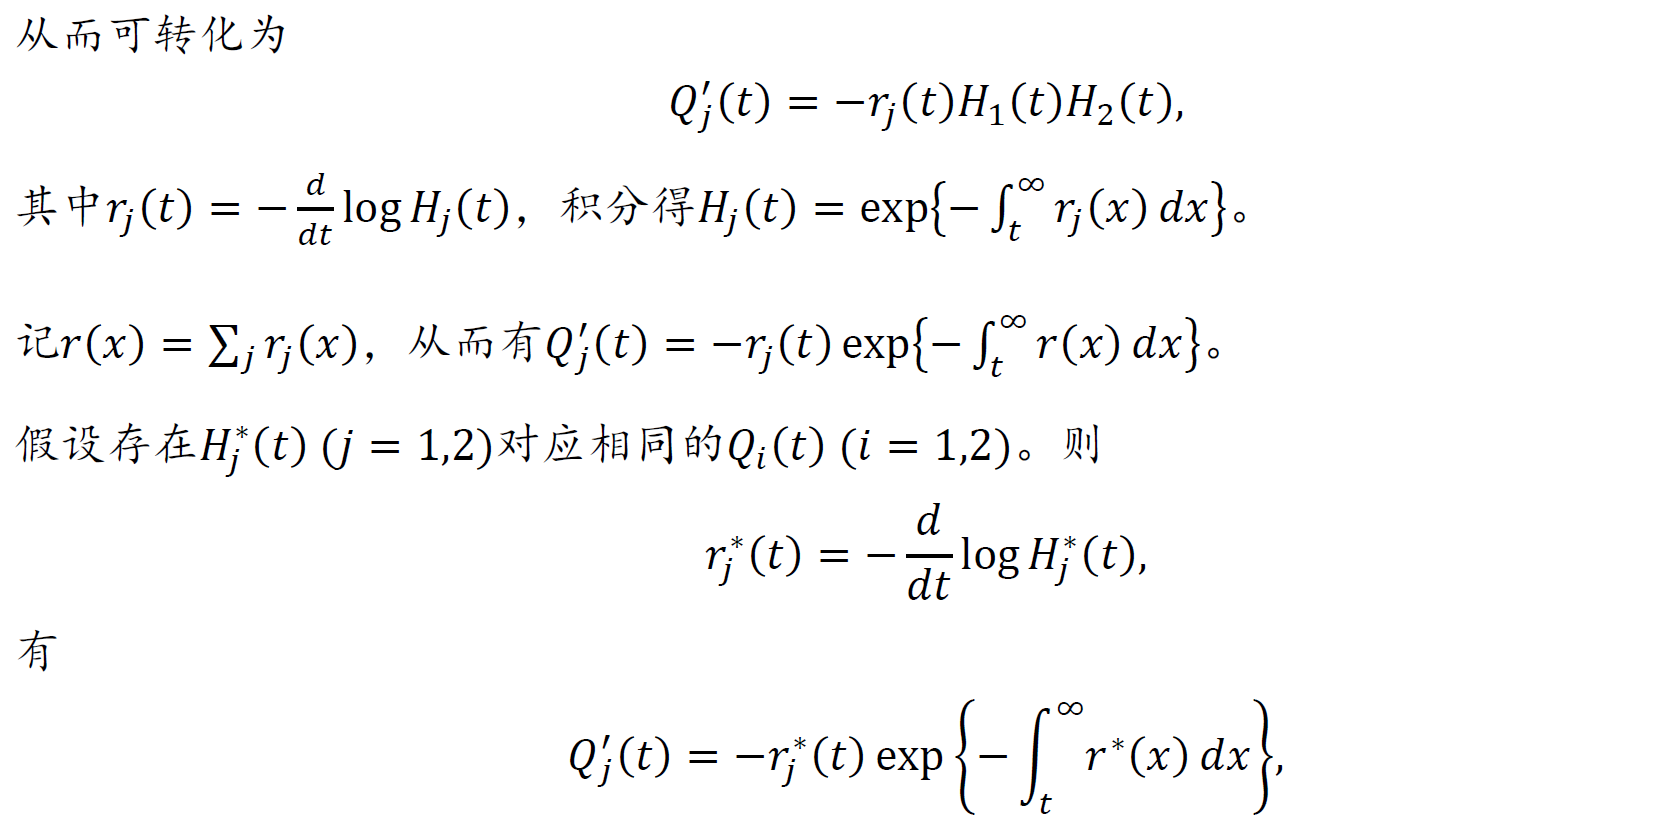
\includegraphics[scale=0.5]{theorem7_3}
\end{frame}
\begin{frame}{Nonidentifiability of a General Nonnormal Roy Model in a Single Cross Section}
	\textbf{Proof:(Cont.)}
	
	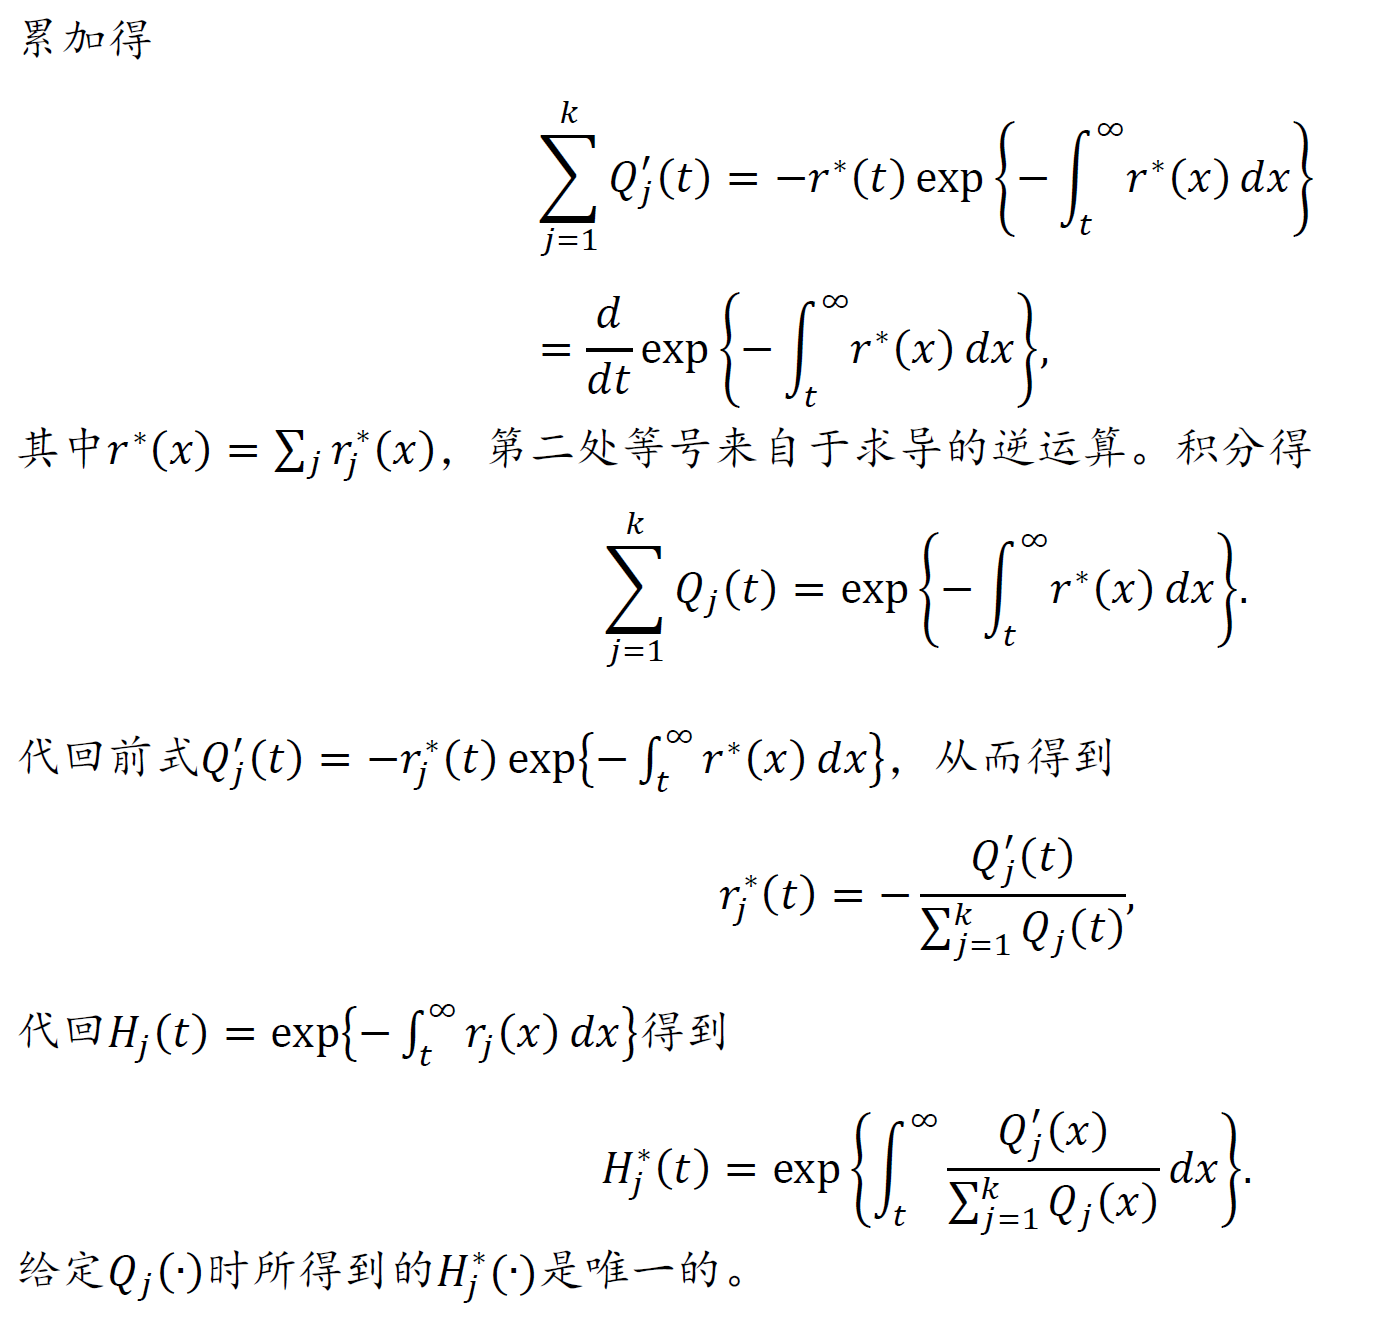
\includegraphics[scale=0.4]{theorem7_4}
\hfill $Q.E.D$
\end{frame}

\begin{frame}{Nonidentifiability of a General Nonnormal Roy Model in a Single Cross Section}
\textbf{Theorem 8:} For any $c<1$, it is always possible to rationalize sectoral wage data in a single cross-section by a \textcolor{red}{two-skill model with correlation greater than c}, provided that $Var[max\{S_1,S_2\}]$ exists.

\bigskip
\textbf{Proof:}

Let $Y$ be the observed wage and let $R$ be an indicator giving the sector associated with that wage. Theorem 7 informs us that any distribution of $(Y,R)$ can be explained by a Roy model with independent skills. On the other hand, imagine that for each $(Y,R)$ we define
	\begin{align}\nonumber
	(S_1,S_2)=\left\{
	\begin{aligned}
	&(Y,Y-\varepsilon),\quad &if\quad R=1,\\
	&(Y-\varepsilon,Y),\quad &if\quad R=2.
	\end{aligned}\right.
	\end{align}
The correlation (provided that it exixts) between $S_1$ and $S_2$ constructed in this manner will depebd on $\varepsilon$, but it can be made arbitrarily close to $1$ by making $\varepsilon$ close to $0$. The theorem naturally follows.\hfill $Q.E.D.$


\end{frame}
%------------------------------------------------

\subsection{Identification from Multi-market Data in a General Nonnormal Roy Model}
\begin{frame}{Identification from Multi-market Data in a General Nonnormal Roy Model}
	\begin{itemize}
		\item These negative conclusions can be reversed with access to data on earnings distributions from markets with \textit{the same distributions of skills but different relative skill prices}.
		\bigskip
		\item With \textcolor{red}{sufficient price variation}, it is possible to identify the population skill distribution
		\item [-] {[Theorem 9]} \textit{even if an agent's sectoral choice is unknown;}
		\item [-] {[Theorem 10]} \textit{even if earnings in one sector are not observed.}
		\item {[Theorem 11]} Access to \textcolor{red}{panel data} greatly reduces the required amount of price variation.
		\item {[Theorem 12]} Access to \textcolor{red}{regressors} that affect the location of the log-skill distribution substitutes for price variation and secures identification in a \textcolor{red}{single cross-section}.
	\end{itemize}
\end{frame}

\begin{frame}{Identification from Multi-market Data in a General Nonnormal Roy Model}
	\textbf{Theorem 9:}  Let $S_1$ and $S_2$ be positive random variables with distribution function $F(s_1,s_2)$. If we only observe $Z=max\{S_1,\pi_2 S_2\}$ and $\pi_2$ takes all possible values in the interval $(0,\infty)$, then $F$ is identifiable.

\bigskip
	\textbf{Proof:}
	
	By assumption we know $Pr(max\{S_1,\pi_2 S_2\}\leq x)$ for all $x$ and $\pi_2$, but
	\begin{equation}\nonumber
	\begin{aligned}
		\{max\{S_1,\pi_2S_2\}\leq x\}&=\{S_1\leq x,\pi_2S_2\leq S_1\}\cup \{\pi_2S_2\leq x,S_1\leq \pi_2S_2\} \\
		&=\{S_1\leq x,S_2\leq x/\pi_2\},
	\end{aligned}
	\end{equation}
so for any $s_1,s_2>0$ we have (setting $x=s_1$ and $\pi_2=s_1/s_2$),
	\begin{equation}\nonumber
	\begin{aligned}
	F(s_1,s_2)&=Pr(S_1\leq s_1,S_2\leq s_2)=Pr(S_1\leq s_1,S_2\leq s_1/\pi_2)\\
	&=Pr(max\{S_1,\pi_2S_2\}\leq x),
	\end{aligned}
	\end{equation}
which completes the proof.\hfill $Q.E.D.$
\end{frame}


\begin{frame}{Identification from Multi-market Data in a General Nonnormal Roy Model}
\textbf{Theorem 10:}  If we observe the distribution of $Z$ given by
	\begin{align}\nonumber
		Z=\left\{
		\begin{aligned}
		&\pi_2S_2\quad &if \quad S_1<\pi_2S_2,\\
		&0 \quad &if \quad S_1\geq \pi_2S_2.
		\end{aligned}\right.
	\end{align}
and $\pi_2$ traverses the interval $(0,\infty)$, then $F(S_1,S_2)$ is identified from \textcolor{red}{multimarket data on aggregate earnings}.

\bigskip
\textbf{Proof:}

Let $s_1,$ $s_2$ be given. We will then show that we can find $F(s_1,s_2)$.

Let $\varepsilon>0$ be given. For given $\pi_2$, we know the probability of events of the type $\{S_1<\pi_2S_2\leq x\}$ for all $x\in (0,\infty)$. This means that we know the probability of the event given by \emph{OAB} in Figure 1. By the same argument, we also know the probability of the event given by the set \emph{OCD}. We therefore know the probability of the difference \emph{DCAB}.
\end{frame}

\begin{frame}{Identification from Multi-market Data in a General Nonnormal Roy Model}
\textbf{Proof:(Cont.)}
By exactly the same reasoning we know the probability of the event \emph{FGED}, and therefore of the event \emph{FGECAB}. If we continue this process, we will converge to a number $\mu$ satisfying
$$F(s_1,s_2)\leq \mu \leq F(s_1+\varepsilon,s_2).$$

Do this for each $\varepsilon$, and the limit as $\varepsilon\to 0$, and we obtain $F(s_1,s_2)$.\hfill $Q.E.D.$
\end{frame}

\begin{frame}{Identification from Multi-market Data in a General Nonnormal Roy Model}
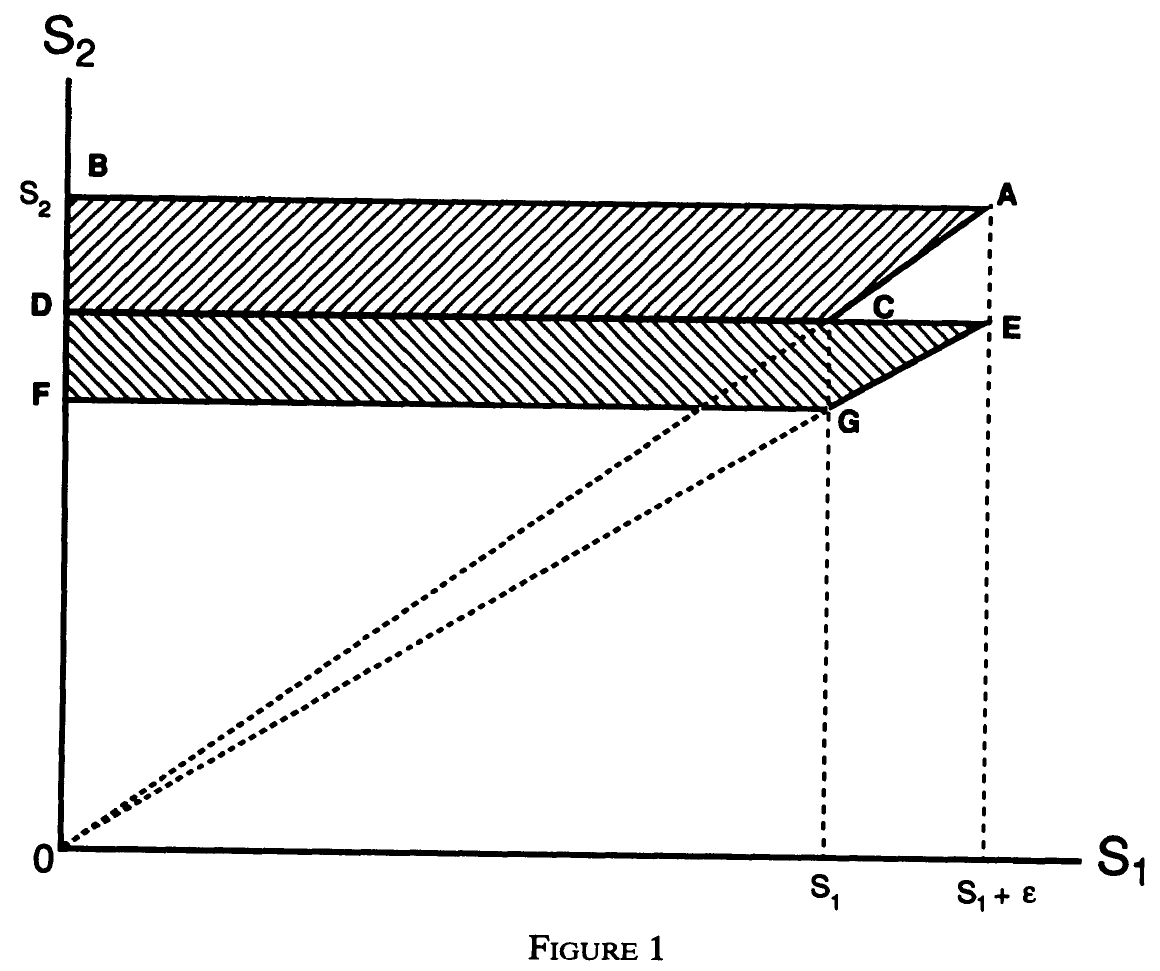
\includegraphics[scale=0.2]{figure1}
\pause
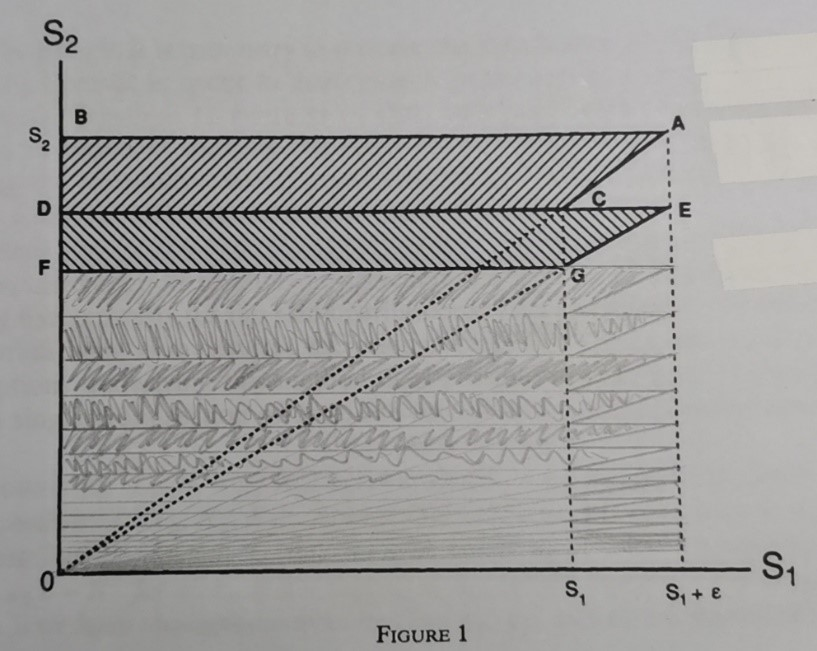
\includegraphics[scale=0.6]{figure2}
\end{frame}


\begin{frame}{Identification from Multi-market Data in a General Nonnormal Roy Model}
\textbf{Theorem 11:}  Suppose that we have \textcolor{red}{panel data} on aggregate earnings of individuals and that individual skills do not change over time. If we observe $(Z,Z' )=(max\{S_1,\pi_2 S_2\},max\{S_1,\pi_2'S_2\})$ for $\pi_2<\pi_2'$, then we can identify $F(s_1,s_2)$ over the region $\pi_2s_2\leq s_1\leq \pi_2's_2$.

\bigskip
\textbf{Proof:} By hypothesis we know $Pr(Z'\leq z',Z\leq z)$ for all $z'$, $z$. Let $s_1,s_2>0$ be given such that $\pi_2s_2\leq s_1\leq \pi'_2s_2$. Now over this region
	\begin{equation}\nonumber
	\begin{aligned}
	F(s_1,s_2)&=Pr(S_1\leq s_1,S_2\leq s_2)\\
	&=Pr(S_1\leq s_1,S_1\leq \pi'_2s_2,S_2\leq s_2,S_2\leq s_1/\pi_2)\\
	&=Pr(S_1\leq s_2,\pi_2S_2\leq s_1,S_1\leq \pi'_2s_2,\pi'_2S_2\leq \pi'_2s_2)\\
	&=Pr(max\{S_1,\pi_2S_2\}\leq s_1,max\{S_1,\pi'_2S_2\}\leq \pi'_2s_2)
	\end{aligned}
	\end{equation}
which, by hypothesis, is known. Hence $F(s_1,s_2)$ is identified for all $\pi_2s_2\leq s_1\leq \pi'_2s_2$.\hfill $Q.E.D.$
\end{frame}

\begin{frame}{Identification from Multi-market Data in a General Nonnormal Roy Model}
	\textbf{Theorem 12:} Let $S_1=g_1(X_1,X_0)+\varepsilon_1$ and $S_2=g_2 (X_2,X_0 )+\varepsilon_2$ where $(\varepsilon_1,\varepsilon_2)$ is independent of $(X_0,X_1,X_2 )$. Assume that
	\begin{itemize}
		\item (a) $(\varepsilon_1,\varepsilon_2)$ is continuously distributed with distribution function $G$ and support equal to $R^2$;
		\item (b) $support(g_1 (X_1,x_0 ),g_2 (X_2,x_0 ))=R^2$ for all $x_0$ in the support of $X_0$;
		\item (c) marginal distributions of $\varepsilon_1$ and $\varepsilon_2$ both have medians equal to $0$.
	\end{itemize}
	Then $g_1$, $g_2$, and $G$ are identified.
\end{frame}

\begin{frame}{Identification from Multi-market Data in a General Nonnormal Roy Model}
\textbf{Proof:} By assumption we know
	\begin{equation}\nonumber
	\begin{aligned}
	(A)\qquad Pr(S_1,S_2)=Pr(g_1(x_1,x_0)&+\varepsilon_1>g_2(x_2,x_0)+\varepsilon_2),\\
	(B) \qquad Pr(S_1\leq y,S_1>S_2)=Pr(&g_1(x_1,x_0)+\varepsilon_1\leq y,\\
	&g_1(x_1,x_0)+\varepsilon_1>g_2(x_2,x_0)+\varepsilon_2),\\
	(C) \qquad Pr(S_2\leq y,S_2\geq S_1)=Pr(&g_2(x_2,x_0)+\varepsilon_2\leq y),\\
	&g_2(x_2,x_0)+\varepsilon_2>g_1(x_1,x_0)+\varepsilon_1),
	\end{aligned}
	\end{equation}
for all $(x_0,x_1,x_2)$ in the support of $(X_0,X_1,X_2)$ and for all $y$.

Fix $x_0$. Let $\bar{x_1}$ and $\bar{x_2}$ be in the support of $X_1$ and $X_2$, respectively. From $(A)$, we can then find
	\begin{equation}\nonumber
	\begin{aligned}
	\{(x_1,x_2):&Pr(g_1(x_1,x_0)+\varepsilon_1>g_2(x_2,x_0)+\varepsilon_2)\} \\
	&=Pr(g_1(\bar{x_1},x_0)+\varepsilon_1>g_2(\bar{x_2},x_0)+\varepsilon_2)\\
	&=\{(x_1,x_2):g_1(x_1,x_0)+l=g_2(x_2,x_0)\}
	\end{aligned}
	\end{equation}
for some unknown constant $l$.
\end{frame}

\begin{frame}{Identification from Multi-market Data in a General Nonnormal Roy Model}
\textbf{Proof:(Cont.)}

For any point in that set, we can use $(B)$ to find
$$Pr(g_1(x_1,x_0)+\varepsilon_1 \leq y,\varepsilon_1>\varepsilon_2+l)$$
for all $y$. This identifies $g_1(\cdot,x_0)$ except for an additive constant. In a similar way, $g_2(\cdot,x_0)$ is identified (except for an additive constant). $G$ is then identified by Theorem 9, except for the location. The location of $G$ is determined by exploiting the fact that the medians of $\varepsilon_1$ and $\varepsilon_2$ are zero. Having determined the location of $G$, we can determined the additive constants in $g_1(\cdot,x_0)$ and $g_2(\cdot,x_0)$.

\medskip
Since $x_0$ was arbitrary, this completes the proof.\hfill $Q.E.D.$
\end{frame}


%------------------------------------------------
\begin{frame}{Summary}
	\begin{itemize}
		\item This paper derive a general class of nonnormal models for which the main conclusion of the Roy model remains valid. It assumes that skills can be decomposed into two components: a log concave random variable and an independent, additive component that can be freely specified. \textit{Selection depends on the log concave component but not on the other component.}

	\end{itemize}
\end{frame}
\begin{frame}{Summary}
	\begin{itemize}
		\item Identifiability is necessary for consistent estimation of the Roy model. This paper only investigate the necessary first step.
		\item [-] \textit{Under Roy's normality assumptions}, it is possible to recover underlying skill distributions from a single cross-section of earnings.
		\item [-] The strong identification results \textit{vanish in a general nonnormal model}, where any single cross-section distribution of wages can be rationalized by a model with independent, positively correlated or negatively correlated skills.
		\item [-] Access to data from \textit{markets with different relative skill prices} facilitates identification; panel data further helps.
		\item [-] With available independent regressors and relative assumptions, \textit{cross-section variation in regressors can substitute for multimarket variation in skill prices}.
	\end{itemize}
\end{frame}
%--------------

%------------------------------------------------

\begin{frame}
\Huge{\centerline{\textit{The End}}}
\end{frame}
%----------------------------------------------------------------------------------------
\section{Appendix}
\begin{frame}{Appendix}
\textbf{Proposition 1:} If $D$ is a \textit{log concave random variable}, then
$$0\leq \frac{\partial E[D|D>d]}{\partial d}\leq 1 $$
$$0\leq \frac{\partial E[D|D\leq d]}{\partial d}\leq 1 $$
and
$$\frac{\partial Var[D|D>d]}{\partial d}\leq 0 $$
$$\frac{\partial Var[D|D\leq d]}{\partial d}\geq 0 $$
\end{frame}
\begin{frame}
	\textbf{Proof of Proposition 1:}
	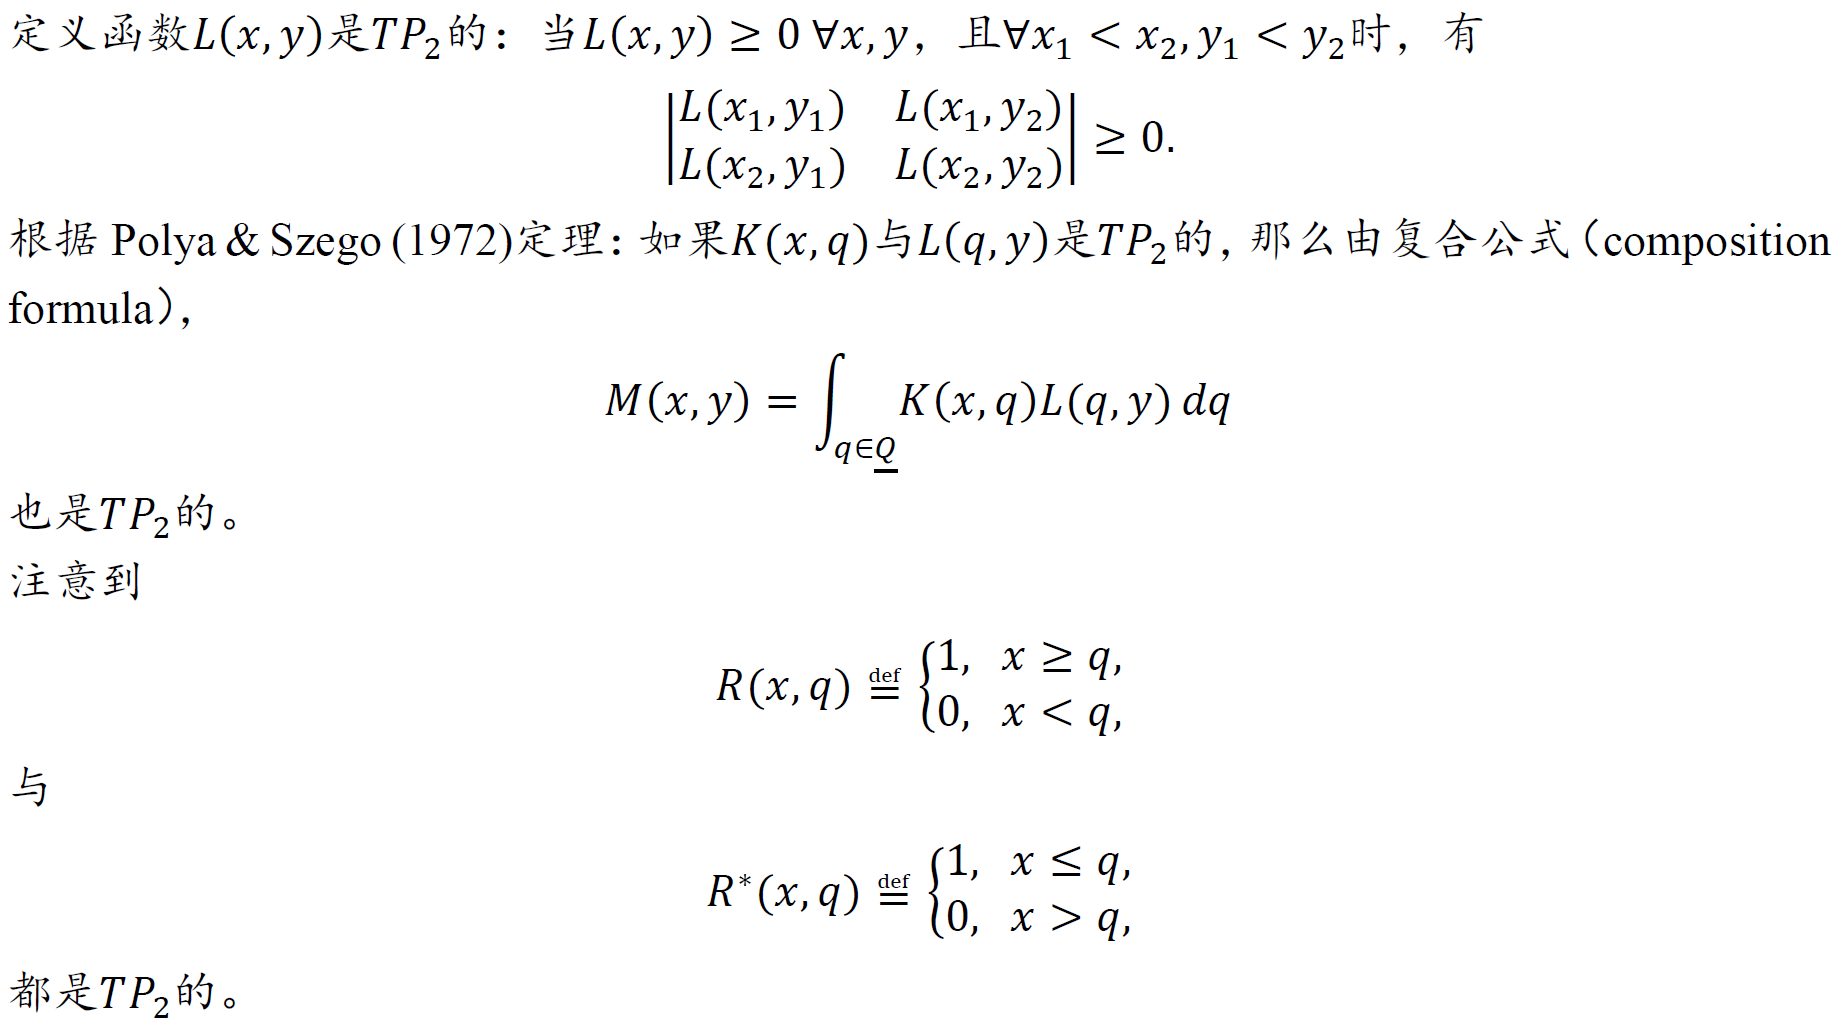
\includegraphics[scale=0.5]{proposition1_1}
\end{frame}
\begin{frame}
	\textbf{Proof of Proposition 1:(Cont.)}
	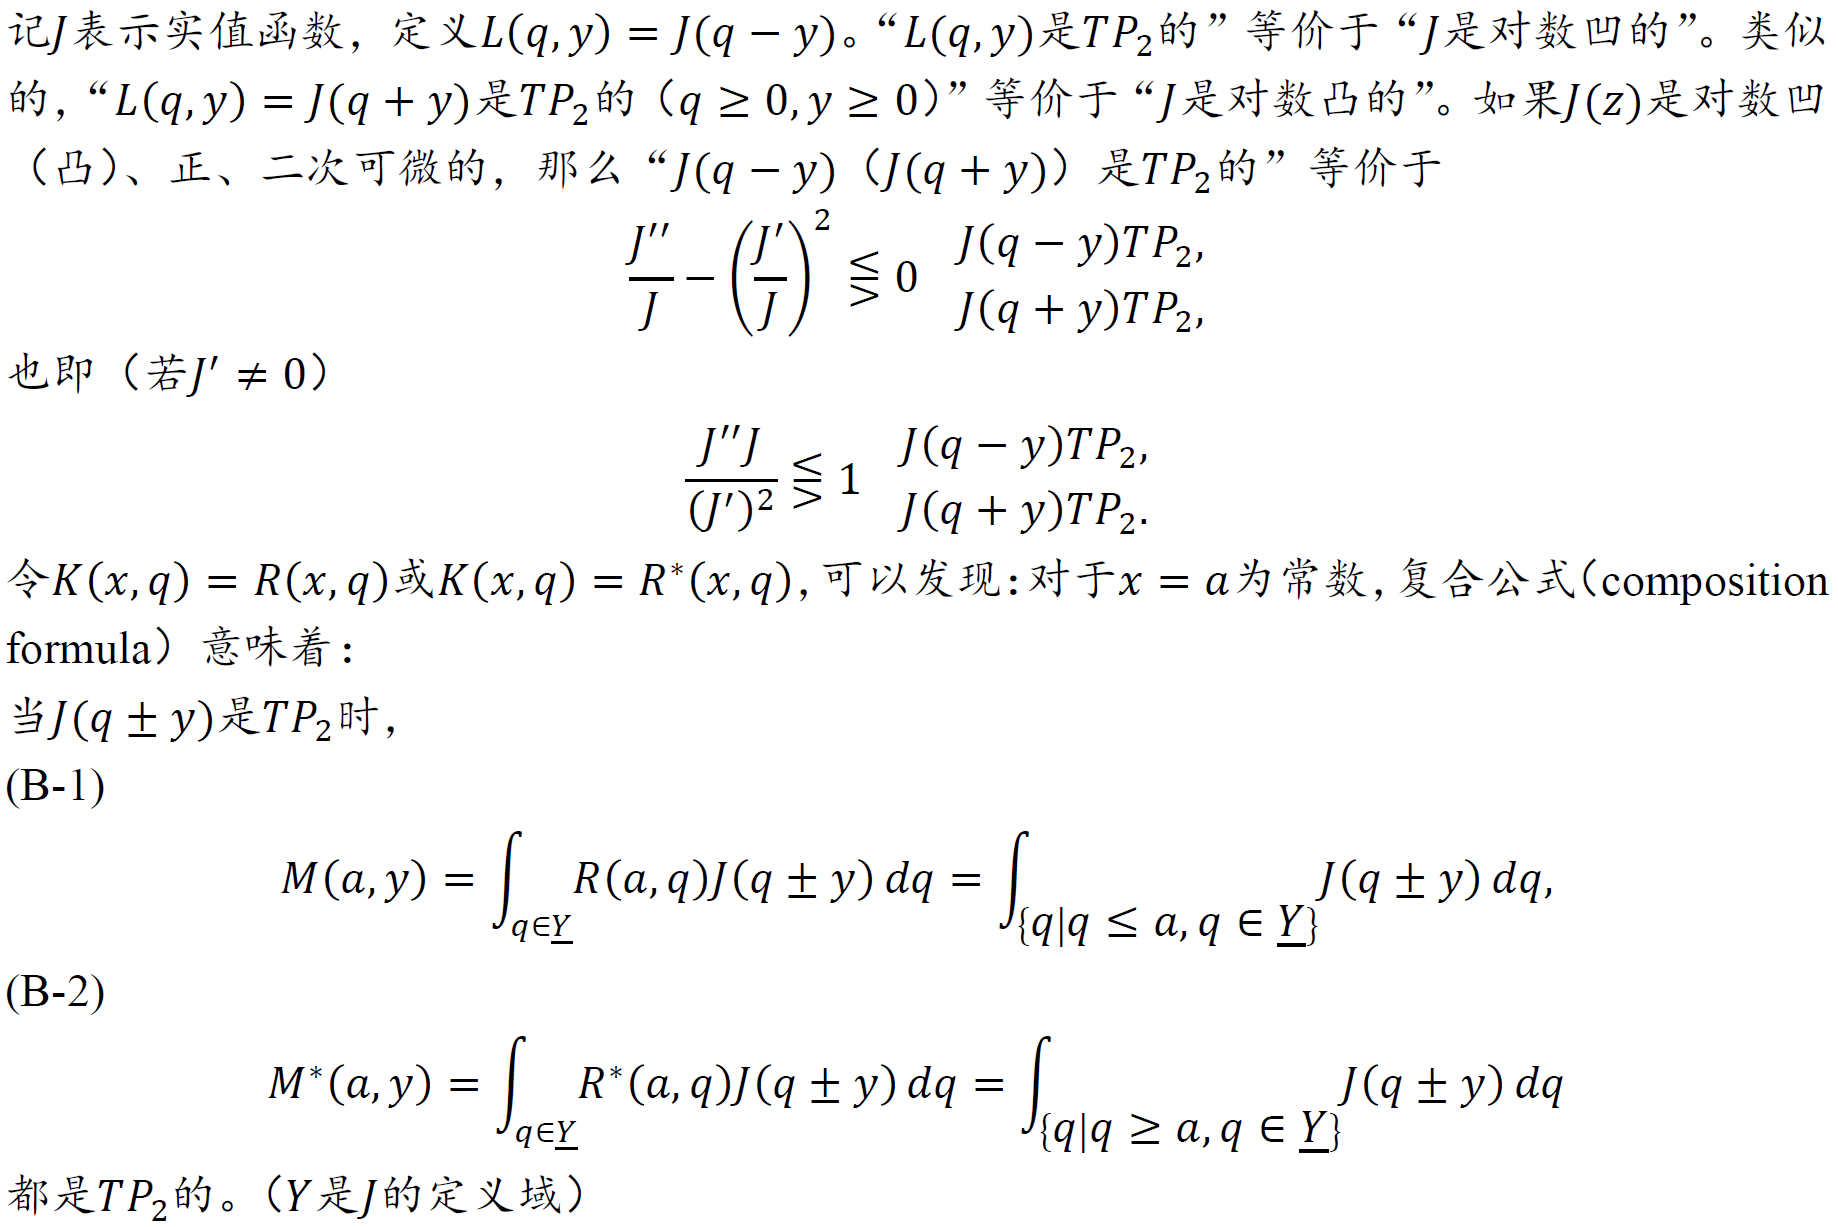
\includegraphics[scale=0.5]{proposition1_2}
\end{frame}
\begin{frame}
	\textbf{Proof of Proposition 1:(Cont.)}
	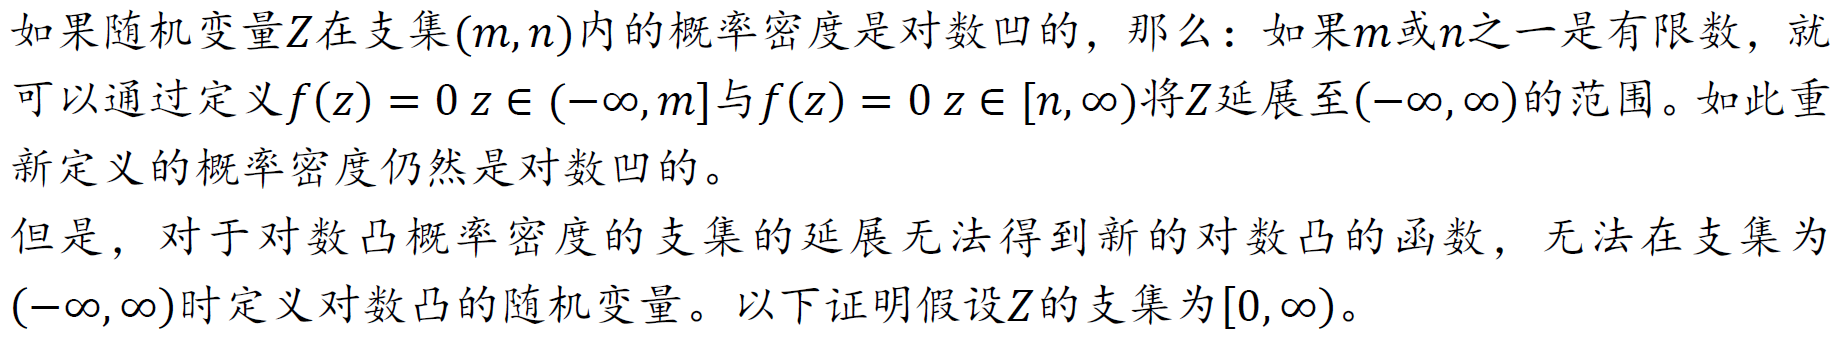
\includegraphics[scale=0.5]{proposition1_3}
\end{frame}
\begin{frame}
	\textbf{Proof of Proposition 1:(Cont.)}
	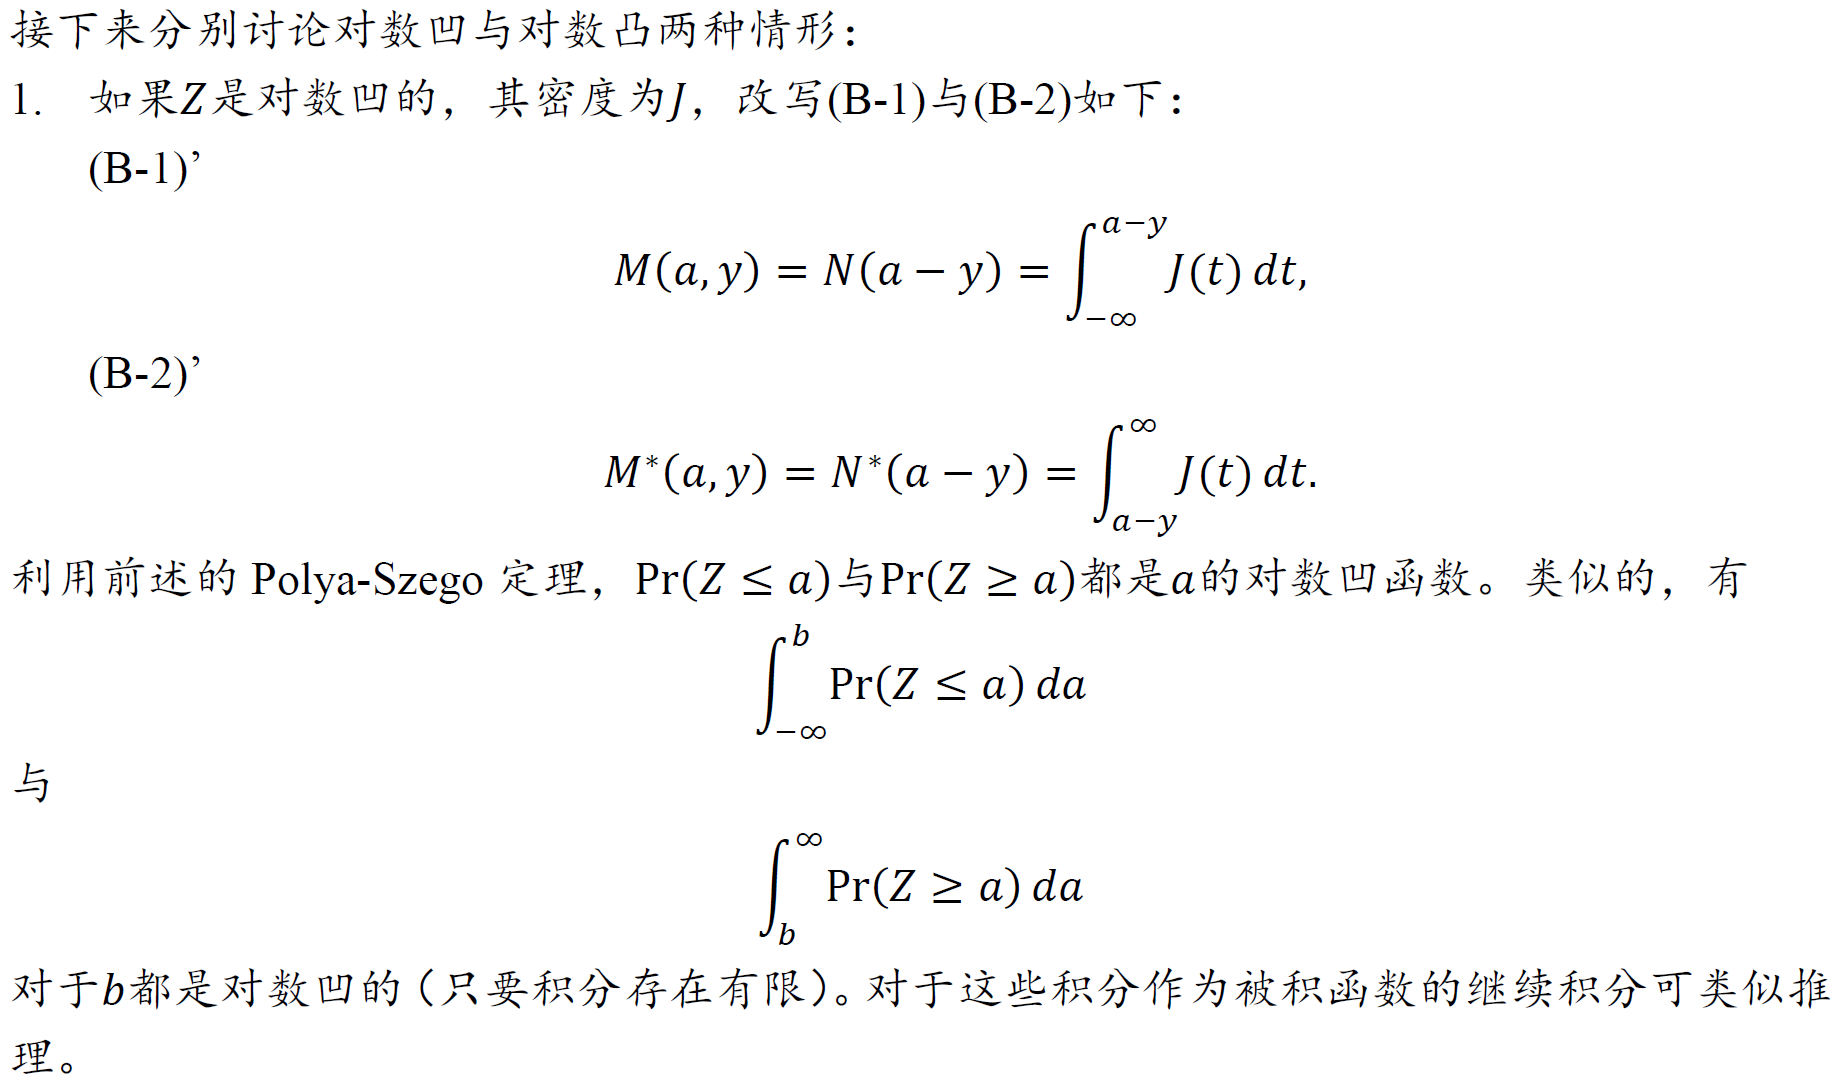
\includegraphics[scale=0.5]{proposition1_4}
\end{frame}
\begin{frame}
	\textbf{Proof of Proposition 1:(Cont.)}
	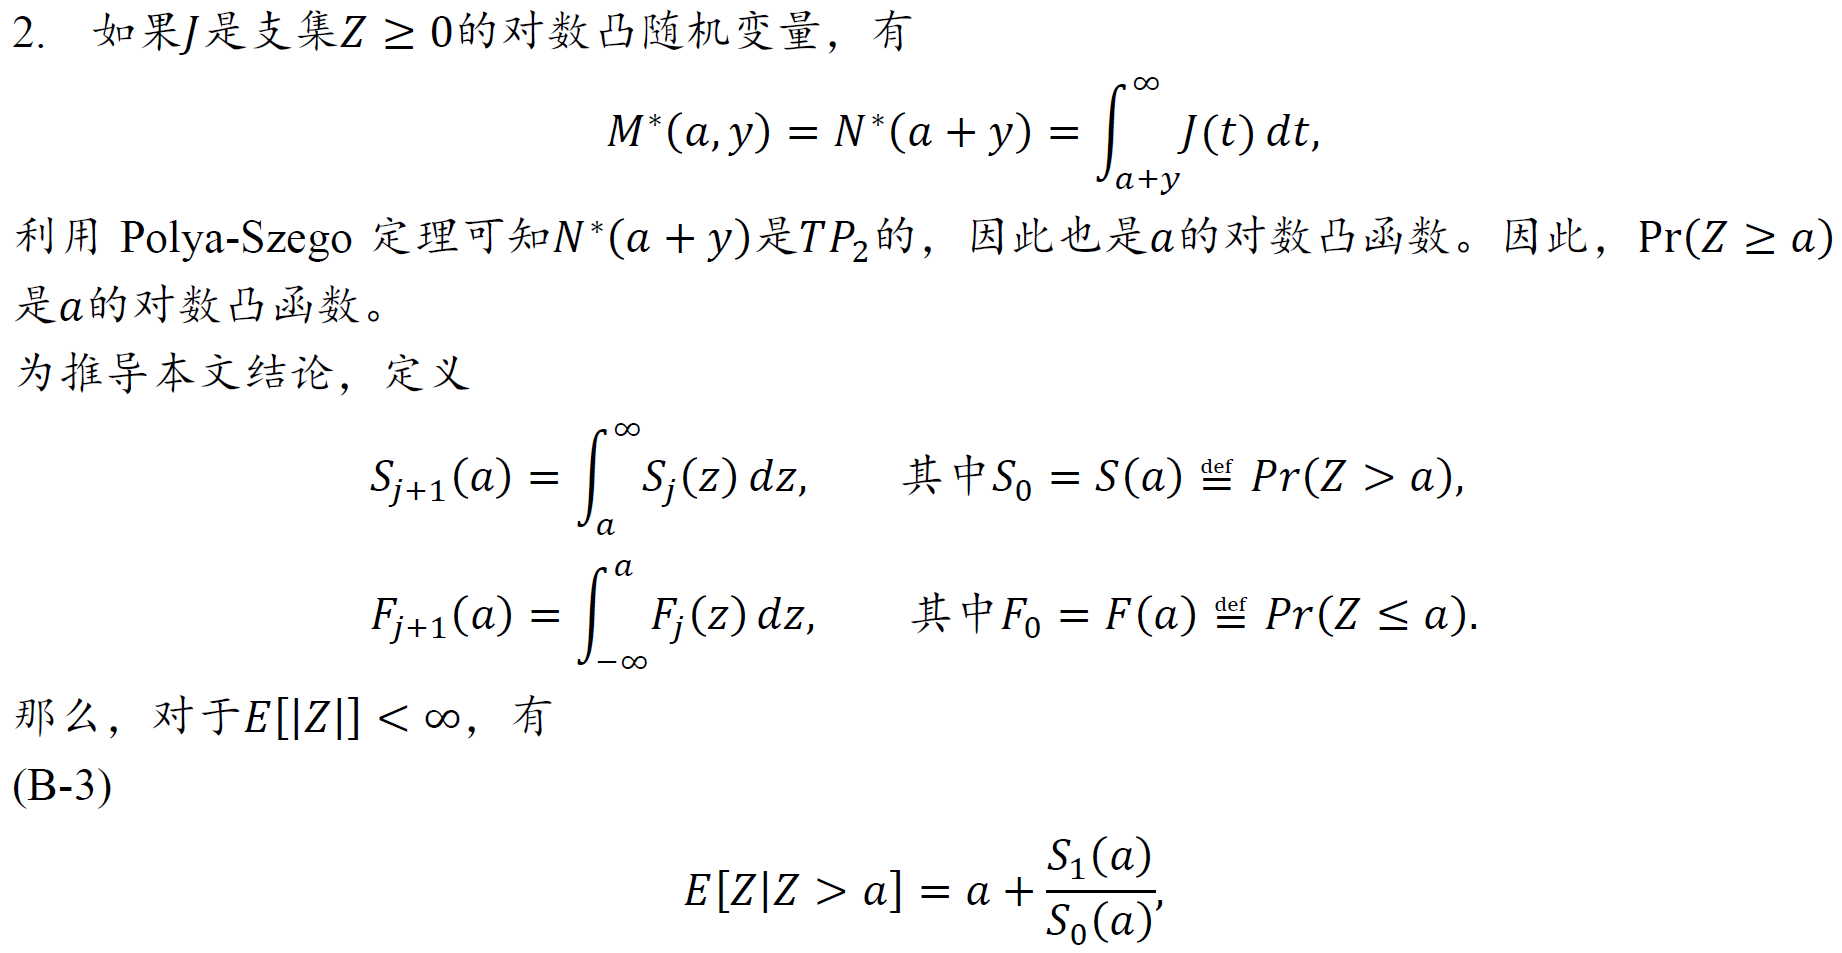
\includegraphics[scale=0.5]{proposition1_5}
\end{frame}
\begin{frame}
	\textbf{Proof of Proposition 1:(Cont.)}
	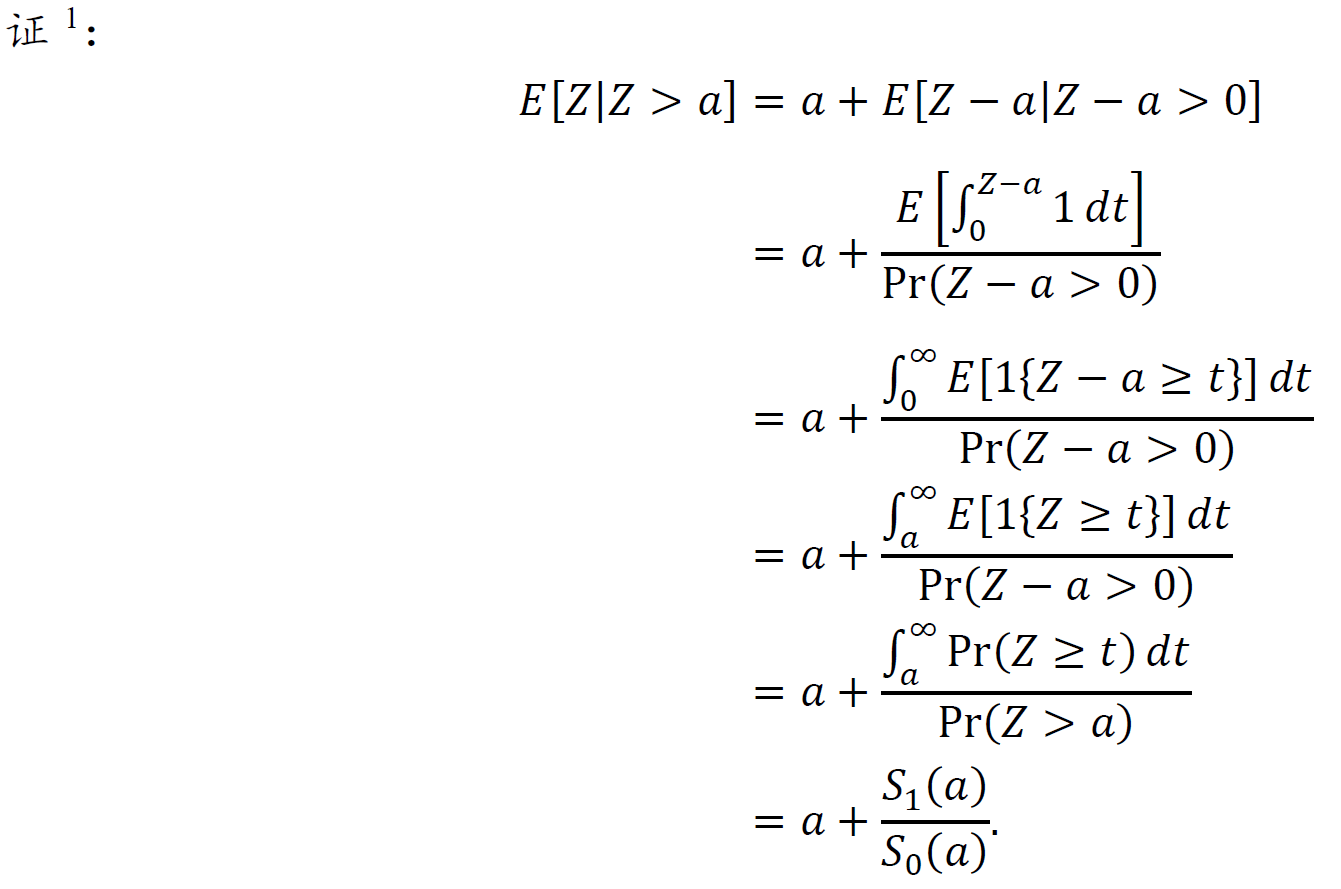
\includegraphics[scale=0.5]{proposition1_6}
\end{frame}
\begin{frame}
	\textbf{Proof of Proposition 1:(Cont.)}
	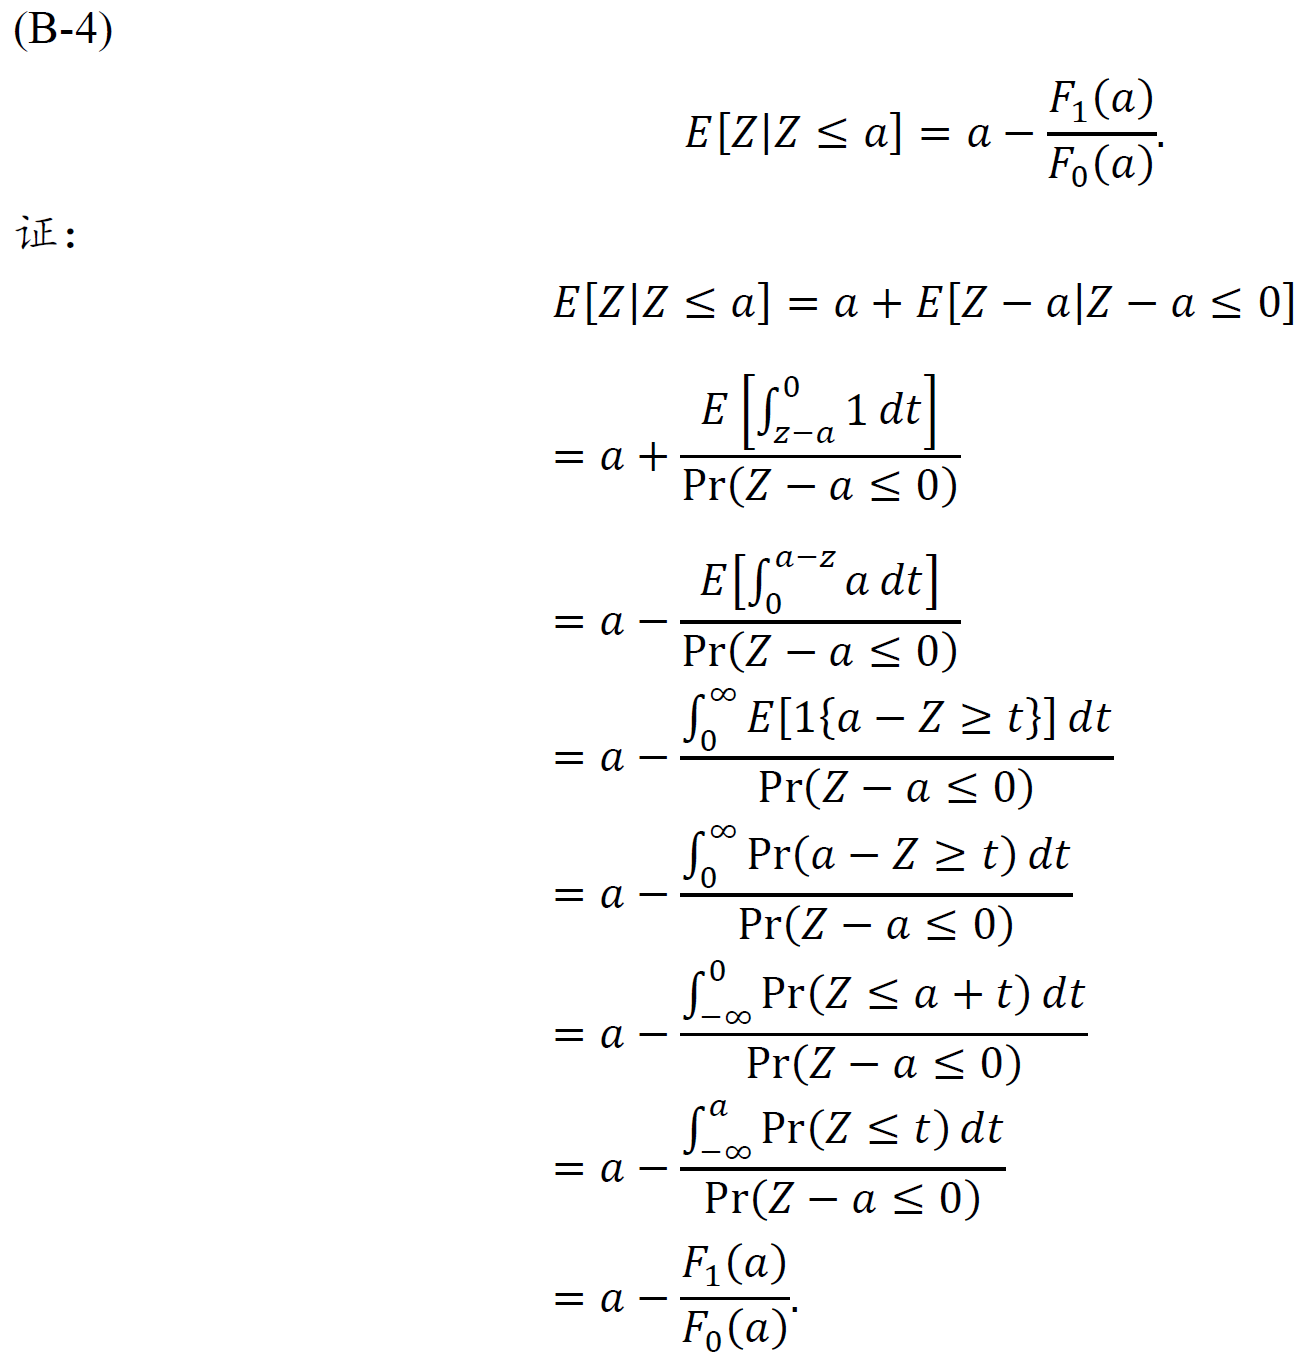
\includegraphics[scale=0.47]{proposition1_7}
\end{frame}
\begin{frame}
	\textbf{Proof of Proposition 1:(Cont.)}
	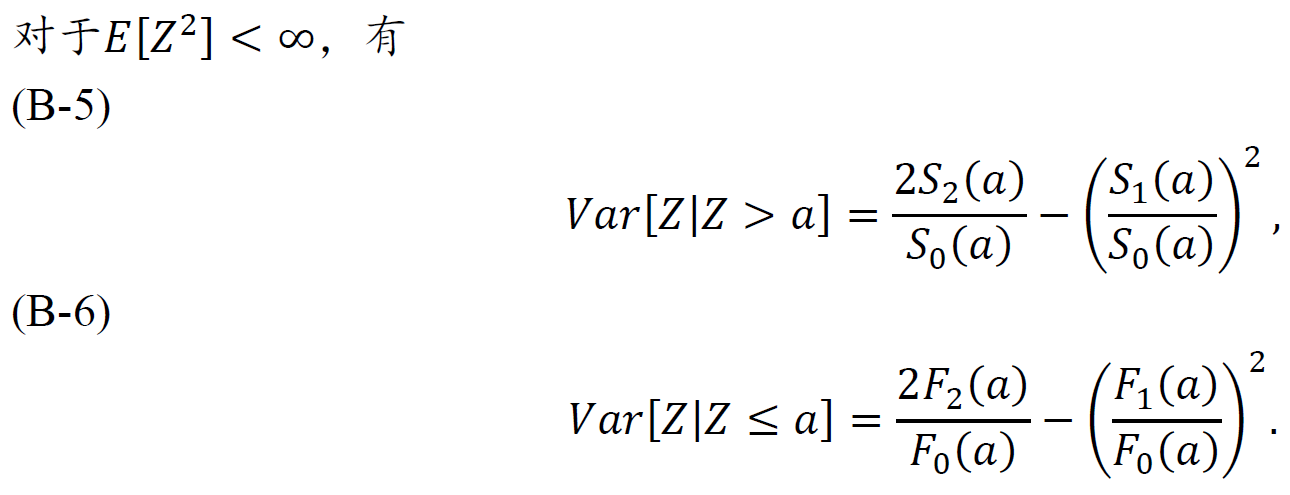
\includegraphics[scale=0.5]{proposition1_8}
\end{frame}
\begin{frame}
	\textbf{Proof of Proposition 1:(Cont.)}
	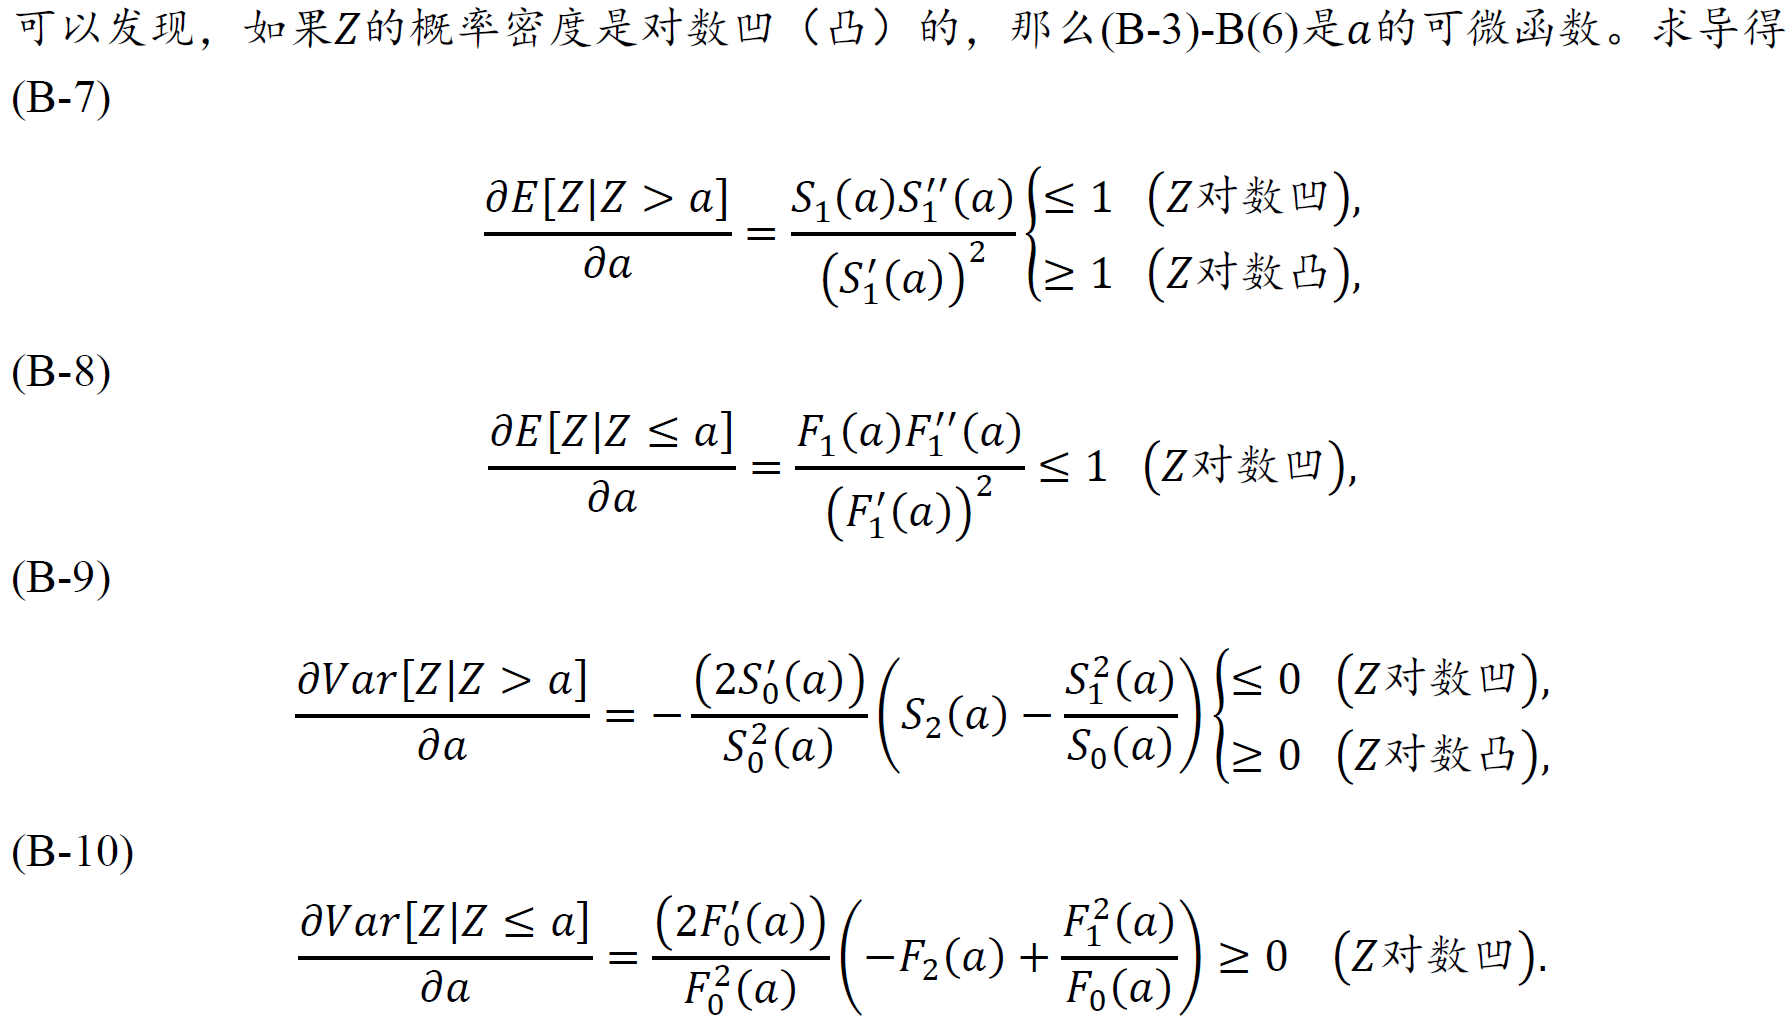
\includegraphics[scale=0.5]{proposition1_9}
\end{frame}







\end{document} 